\documentclass[11pt,a4paper]{article}
\usepackage[margin=2.5cm]{geometry}
\usepackage{amsmath,amssymb,physics}
\usepackage{booktabs}
\usepackage{hyperref}
\usepackage{enumitem}
\usepackage{caption}
\usepackage{verbatim}
\usepackage{tcolorbox}
\tcbuselibrary{skins,breakable}

% Coloured result boxes
\newtcolorbox{resultbox}[1][]{enhanced,breakable,
  colback=blue!4!white,colframe=blue!40!black,
  fonttitle=\bfseries,title={#1},boxrule=0.6pt,arc=4pt}
\newtcolorbox{gapbox}[1][]{enhanced,breakable,
  colback=orange!6!white,colframe=orange!60!black,
  fonttitle=\bfseries,title={#1},boxrule=0.6pt,arc=4pt}

\hypersetup{
    colorlinks=true,
    linkcolor=blue,
    citecolor=blue,
    urlcolor=blue
}
\newcommand{\seriesname}{Saturated Superfluid Vacuum}
\newcommand{\papernumber}{I}
\title{\textbf{\seriesname~\papernumber}\\[0.4em]
\large Topological Defects in a Saturated Superfluid Vacuum:\\
The Geometric Origin of Matter and\\
the $\alpha$-Harmonic Mass Ladder}
\author{Stig Norland \\ Independent Researcher \\ Bergen, April 2026}
\date{}

\begin{document}

\maketitle

\begin{abstract}
We propose that the physical vacuum is a compressible, inviscid superfluid near
saturation density --- a single postulate from which the structure of fundamental
particles and constraints on the fine-structure constant emerge.  Particles are
stable topological defects: quantised toroidal vortex rings (leptons) and spherical
breathers stabilised by trefoil vortex skeletons (baryons).

From the logarithmic Schr\"{o}dinger Lagrangian we derive three results from first
principles.  First, the sound-speed condition $c_s = c$ fixes the stiffness parameter
$b = m_0 c^2/(2\rho_0)$ and the healing length $\xi = \hbar/(m_0 c)$.  Second,
minimisation of the three-term vortex-ring energy functional over torus radius $R$
and core radius $a$ yields the unique equilibrium $R_e^* = \xi/\alpha$, from which
the vacuum density $\rho_0$ is fixed via the Lamb formula with no free parameters
beyond the two empirical inputs $m_e$ and $\alpha$.  Third, the ratio of the
chiral-shear speed $c_\perp$ to the sound speed $c_s$ identifies $\alpha \approx
1/137$ as a geometric property of the medium.

These results establish the base energy scale $\mu_0 \equiv m_e c^2/\alpha \approx
70\,\text{MeV}$ as the energy of a minimal vortex filament segment of the electron
Compton circumference.  The charged pion, as the minimal vortex-antivortex bound
state carrying two winding numbers, then has mass $m_{\pi^\pm} = 2\mu_0$, agreeing
with CODATA at $0.34\%$.

Direct 3D toroidal Bogoliubov--de~Gennes projection with chiral-shear coupling,
developed in this paper, identifies the dynamical mechanism behind the muon
rung: the lowest hybrid of the $m_\varphi=0$ core-breathing mode with the
$m_\varphi=\pm1$ Kelvin centerline sector in the helicity basis, coupled through
the second variation of $\mathcal{L}_\perp$.  Driven-response calculations
confirm a selection rule: core-breathing boundary drives preferentially excite
the $(3/2)\mu_0$ tongue identified with the muon, while Kelvin helicity drives
preferentially excite the $2\mu_0$ tongue identified with the charged pion.
In the present meridional projection the muon eigenfrequency falls in the range
$\omega_\mu/\omega_c\in[0.19,0.23]$ depending on meridional domain size,
bracketing the observed value $0.207\,\omega_c$ without yet resolving to a
single number; thin-ring analytic closure is required for a sharp prediction
and is deferred to Paper~II.  For the proton, the empirical scaling
$m_p c^2 = N_Y\!\cdot\!F\!\cdot\!\mu_0$ with $N_Y\approx3.007$ and form factor
$F\approx4.4$--$4.47$ at the inter-strand half-spacing cutoff
$R\approx1.18\,\xi$ yields $m_p\approx 927$--$941\,\text{MeV}$
($1.2\%$--$0.3\%$ from CODATA, depending on the cutoff convention).
The neutron is given a structural derivation as the surface-locked composite
$\mathcal{N}=\mathcal{T}\cup_{\Sigma_p}\mathcal{E}$ of the proton trefoil and
an electron torus compressed onto the breather skin: charge, spin,
spin-statistics composition, and baryon/lepton number follow without fitting
from boundary-framed vs bulk-framed defect classification, and the mass
splitting decomposes as $\Delta E = m_e c^2 + \Delta E_{\rm surf}$ with
$\Delta E_{\rm surf}$ identified as the $\beta$-decay endpoint
$0.782\,\text{MeV}$; quantitative pinning of $\Delta E_{\rm surf}$ inherits the
proton-closure work and is tracked under issue~\#30.

Two empirical inputs ($m_e$, $\alpha$) are used.  The remaining predictions
are consistent with the observed lepton and light-hadron spectrum at the
$\lesssim 1.5\%$ level under the present effective theory, with explicit
dependence on the regularisation cutoff $R$ and the meridional domain size
$L_{\rm box}$ documented in the body.  A dedicated Claim Status section
(\S\ref{sec:claim-status}) tags every quantitative claim as
\textit{derived}, \textit{structural}, \textit{candidate}, or
\textit{ansatz}, and links each candidate-grade claim to the consolidated tracking
issue~\#30, whose computations would change its status.
The open problems for Paper~II are: thin-ring analytic closure of the
muon eigenfrequency, full 3D minimisation for the proton form factor
(including a cutoff-stability scan for $F(R)$ and a dedicated $N_Y$
cross-grid refinement), and a basis-enrichment programme that
demonstrates the $1/\sqrt{N_{\rm modes}}$ residual scaling proposed
for the muon rung.  The previously headlined $0.3\%$ proton-mass
agreement is the precision at a specific calibration cutoff
$R\approx1.18\,\xi$ and is reframed in this paper as a $\sim$1.5\%
match with documented cutoff sensitivity.
\end{abstract}

\newpage
\tableofcontents
\newpage

%------------------------------------------------------------------
\section{Introduction: The Crisis of Abstraction}
%------------------------------------------------------------------
The Standard Model predicts particle masses, charges and interaction rates with
extraordinary precision, yet it provides no mechanism for \emph{why} these quantities
take their observed values.  Some 19 free parameters---particle masses, coupling
constants, mixing angles---must be inserted by hand.  At the same time, attempts
to quantize gravity perturbatively produce non-renormalizable divergences, and
roughly $95\%$ of the universe's energy content must be assigned to unknown dark
components inferred only from gravitational anomalies.

We propose that this impasse reflects a missing ontological layer.  The vacuum
is not empty: it is a physical substance---a saturated superfluid.  All phenomena
emerge from its hydrodynamics.  This idea has deep roots.  Volovik has shown that
the low-energy physics of superfluid $^3$He reproduces the structure of the
Standard Model, with Lorentz symmetry, gauge bosons, and chiral fermions emerging
as collective excitations~\cite{volovik2003}.  Barcel\'o, Liberati, and Visser
established the analogue-gravity programme: acoustic perturbations of any
irrotational, barotropic fluid obey a curved-spacetime wave equation, so
gravitational phenomenology emerges from fluid dynamics~\cite{barcelo2011}.
Hu has argued that spacetime itself is an emergent concept from a
more fundamental substrate~\cite{hu2009}.

The present work pursues a specific realisation of this programme: a logarithmic
nonlinear Schr\"{o}dinger (LogSE) field theory for the vacuum order parameter,
supplemented by a chiral-shear term.  Stable topological defects of this
field---toroidal vortex rings and spherical breathers---are identified with
fundamental particles.  The mass spectrum of these defects organises into a
harmonic ladder governed by the fine-structure constant $\alpha\approx1/137$.

This paper is organised as follows.  Section~\ref{sec:postulate} states the
fundamental postulate, derives the equations of motion from the LogSE Lagrangian,
derives the sound speed, and establishes the origin of $\alpha$ from the
chiral-shear coupling.  Section~\ref{sec:matter} establishes the equilibrium vortex geometry and the
vacuum density from the Lamb vortex-ring formula, taking $m_e$ and $\alpha$
as empirical inputs, and presents the proton and neutron models.
Section~\ref{sec:ladder} develops the $\alpha$-harmonic mass ladder, including the
pion (analytically), the muon (dynamically motivated bracket), and the proton
(numerically extracted, cutoff-dependent).  Section~\ref{sec:forces} sketches the emergence of forces.
Sections~\ref{sec:outlook}--\ref{sec:conclusion} give the outlook and conclusions.
Appendices contain the numerical minimisation and the BdG eigenvalue equations
together with their numerical solution.

%------------------------------------------------------------------
\section{The Fundamental Postulate}
\label{sec:postulate}
%------------------------------------------------------------------

The physical vacuum is a continuous, compressible, inviscid superfluid at
near-saturation density $\rho_0$, with background pressure $P_0\gg\rho_0 c^2$.
All known physics emerges from the hydrodynamics of this single medium; no additional
fields or symmetry-breaking mechanisms are required at the foundational level.

The defining characteristics are:

\begin{itemize}
  \item \textbf{Compressibility and high stiffness.}
        The equation of state is such that small density perturbations propagate as
        pressure waves at speed $c_s=\sqrt{\partial P/\partial\rho}$.  At the
        background state, we require $c_s=c$ (the observed speed of light) to be
        constant (Lorentz-invariant in the low-momentum limit).  The condition
        $P_0\gg\rho_0 c^2$ ensures the medium remains far from the
        laminar-to-turbulent transition under ordinary stresses, while still allowing
        topological defects to form under extreme local strain.

  \item \textbf{Inviscid flow.}
        Zero (or exponentially suppressed) viscosity guarantees dissipation-free
        long-range coherence---persistent currents, quantized circulation, and stable
        solitons.  This is the hydrodynamic analogue of unitarity and conservation
        laws.

  \item \textbf{Light as sound.}
        Electromagnetic waves (and massless modes generally) are long-wavelength
        longitudinal/transverse pressure oscillations in the superfluid.  Thus,
        \begin{equation}
          c = c_s(\rho_0)
            = \sqrt{\left.\frac{\partial P}{\partial\rho}\right|_{\rho_0}}.
          \label{eq:sound-speed}
        \end{equation}
        In logarithmic superfluid models (common in SVT literature), the
        pressure-density relation takes the form
        $P\propto-\rho\ln(\rho/\bar{\rho})$~\cite{volovik2003,volovik2001},
        yielding constant $c_s$ at low excitations while allowing deformed
        dispersion at high momenta.

  \item \textbf{Special relativity as emergent hydrodynamics.}
        Objects composed of stable topological defects (vortices/breathers) experience
        length contraction and time dilation as equilibrium responses to motion through
        the medium.  A moving defect induces a wake; to minimise energy/disruption the
        defect contracts in the propagation direction (Lorentz--FitzGerald style).  The
        medium itself remains undetectable in Michelson--Morley-type interferometers
        because the ``ether wind'' is canceled by the defect's own flow field---the drag
        is internal to the object-medium system.
\end{itemize}

This postulate recovers special relativity in the low-velocity, low-excitation limit
without assuming a priori Lorentz symmetry~\cite{volovik2003,barcelo2011}; the
symmetry emerges from the constancy of $c_s$ and the irrotational nature of small
perturbations (potential flow).  At higher energies/momenta, deviations from exact
Lorentz invariance are expected (deformed dispersion relations), consistent with hints
from ultra-high-energy cosmic rays and some quantum-gravity phenomenology~\cite{barcelo2011,zloshchastiev2020}.

%------------------------------------------------------------------
\subsection{Effective Lagrangian and Equations of Motion}
\label{sec:lagrangian}
%------------------------------------------------------------------

The dynamics of the saturated superfluid vacuum are governed by an effective field
theory for the complex order-parameter field $\Psi$ (normalised so
$|\Psi|^2=\rho/\rho_0$).  Following the superfluid-vacuum framework of
Volovik~\cite{volovik2003}, we adopt a logarithmic nonlinear Schr\"{o}dinger
Lagrangian:
\begin{equation}
  \mathcal{L}
  = \frac{i\hbar}{2}\bigl(\Psi^*\partial_t\Psi - \Psi\,\partial_t\Psi^*\bigr)
    - \frac{\hbar^2}{2m_0}|\nabla\Psi|^2
    - V(\rho),
  \label{eq:Lag}
\end{equation}
where the potential is
\begin{equation}
  V(\rho) = -b\,\rho\bigl[\ln(\rho/\bar{\rho})-1\bigr]+V_0,
  \label{eq:pot}
\end{equation}
with $b>0$ a stiffness parameter and $\bar{\rho}$ the saturation density.
Applying the Euler--Lagrange equation to~\eqref{eq:Lag}, using
$\partial V/\partial\Psi^* = (dV/d\rho)\rho_0\Psi$ and
$dV/d\rho = -b\ln(\rho/\bar\rho)$, yields the logarithmic Schr\"{o}dinger
equation (LogSE):
\begin{equation}
  i\hbar\,\partial_t\Psi
  = -\frac{\hbar^2}{2m_0}\nabla^2\Psi
    - b\rho_0\ln\!\left(\frac{\rho_0|\Psi|^2}{\bar{\rho}}\right)\Psi.
  \label{eq:LogSE}
\end{equation}

\textbf{Madelung representation.}
Writing $\Psi=\sqrt{\rho/\rho_0}\,e^{i\theta}$ with superfluid velocity
$\mathbf{v}=(\hbar/m_0)\nabla\theta$, the LogSE~\eqref{eq:LogSE} separates
into real and imaginary parts.  The imaginary part gives the exact continuity
equation
\begin{equation}
  \partial_t\rho + \nabla\cdot(\rho\mathbf{v}) = 0.
  \label{eq:continuity}
\end{equation}
The real part, after dividing by $\rho$, gives an Euler equation
\begin{equation}
  \partial_t\mathbf{v} + (\mathbf{v}\cdot\nabla)\mathbf{v}
  = -\frac{1}{m_0\rho}\nabla P(\rho)
    + \frac{\hbar^2}{2m_0^2}\nabla\!\left(\frac{\nabla^2\!\sqrt{\rho}}{\sqrt{\rho}}\right),
  \label{eq:euler}
\end{equation}
where the pressure follows the logarithmic equation of state
$P(\rho)=b\rho\ln(\rho/\bar\rho)$.  The last term is the quantum-pressure
(Bohm potential), which is negligible at wavelengths $\lambda\gg\xi$;
at those scales the LogSE reduces to a \emph{compressible inviscid fluid}
with logarithmic EOS.  The thermodynamic sound speed
$c_{\rm thermo}=\sqrt{(1/m_0)dP/d\rho|_{\rho_0}}=\sqrt{b/m_0}$ is half the
Bogoliubov result $c_s=\sqrt{2b\rho_0/m_0}$; the discrepancy is resolved by
the coupled amplitude-phase Bogoliubov dispersion, which gives
$\omega^2=c_s^2k^2(1+k^2\xi^2)$ with $c_s=\sqrt{2b\rho_0/m_0}$.

\textbf{Sound speed.}
Linearising around the uniform background $\Psi=1+\eta$, $|\eta|\ll1$,
with $\rho_0=\bar\rho$, the density channel satisfies a wave equation with
phase velocity
\begin{equation}
  c_s = \sqrt{\frac{2b\rho_0}{m_0}}.
  \label{eq:cs}
\end{equation}
Setting $c_s=c$ fixes the stiffness parameter: $b=m_0c^2/(2\rho_0)$.
The healing length (vortex core size) is
\begin{equation}
  \xi = \frac{\hbar}{\sqrt{2m_0 b\rho_0}} = \frac{\hbar}{m_0 c},
  \label{eq:xi}
\end{equation}
i.e., the Compton wavelength of the reference mass $m_0$.

\textbf{Transverse stiffness and the origin of $\alpha$.}
The LogSE admits only irrotational flow at linear order.  To support stable
vortices and a transverse shear channel (necessary for electromagnetism to
emerge as chiral flow gradients), we supplement $\mathcal{L}$ with the
chiral-shear term
\begin{equation}
  \mathcal{L}_\perp
  = -\frac{\lambda\hbar^2}{2m_0\rho_0^2}
    \bigl|(\nabla\times\mathbf{j})\bigr|^2,
  \label{eq:chiral}
\end{equation}
where $\mathbf{j}=(\hbar/2m_0 i)(\Psi^*\nabla\Psi-\Psi\nabla\Psi^*)$
is the probability current and $\lambda>0$ is a dimensionless coupling.
This produces a transverse mode with phase speed $c_\perp(k) \propto k$ at
wavenumber $k$.  Evaluating at the vortex core scale $k\sim1/\xi$ gives
\begin{equation}
  \frac{c_\perp}{c} = \sqrt{\frac{\lambda m_0}{\rho_0}} \equiv \alpha.
  \label{eq:alpha-origin}
\end{equation}
The fine-structure constant $\alpha\approx1/137$ is therefore the ratio of
the transverse shear speed to the longitudinal sound speed in the vacuum at
the core scale.  Equation~\eqref{eq:alpha-origin} fixes the chiral coupling
$\lambda=\alpha^2\rho_0/m_0$; with $\alpha=1/137$ and
$\lambda\approx2000$ (from the numerical minimisation in
Appendix~\ref{app:construction}), this yields
$\rho_0/m_0 = \lambda/\alpha^2 \approx 3.75\times10^7$ as a dimensionless
characterisation of the vacuum state.

\begin{resultbox}[Two derived results]
\begin{enumerate}
  \item The LogSE with potential~\eqref{eq:pot} has longitudinal sound speed
        $c_s=\sqrt{2b\rho_0/m_0}$; setting $c_s=c$ gives $b=m_0c^2/(2\rho_0)$
        and healing length $\xi=\hbar/(m_0c)$.
  \item With the chiral-shear term~\eqref{eq:chiral}, the transverse phase
        speed at the core scale is $c_\perp=c\sqrt{\lambda m_0/\rho_0}$;
        identifying $c_\perp/c=\alpha$ fixes $\lambda=\alpha^2\rho_0/m_0$.
\end{enumerate}
These are the only two results needed to motivate $\mu_0=m_ec^2/\alpha$ as
the natural flux-tube energy scale (see \S\ref{sec:ladder}).
\end{resultbox}

This Lagrangian admits \textbf{quantised circulation}
$\oint\mathbf{v}\cdot d\mathbf{l}=nh/m_0$ (Onsager--Feynman) and supports stable
topological defects.  Stable defect geometries are constructed and their
mass assignments established in Sections~3--4.


%------------------------------------------------------------------
\section{The Geometric Origin of Matter}
\label{sec:matter}
%------------------------------------------------------------------
Matter forms when the medium is stressed beyond its laminar limit, collapsing into
stable topological defects (vortices).

%------------------------------------------------------------------
\subsection{The Electron (The Torus)}
\label{sec:electron}
%------------------------------------------------------------------
The electron is modelled as a quantized toroidal vortex ring in the saturated
superfluid vacuum---a stable, self-sustaining topological defect with finite size.

\begin{itemize}
  \item \textbf{Spin.}
        The intrinsic angular momentum arises from the quantized circulation around
        the toroidal path:
        \begin{equation}
          \oint\mathbf{v}\cdot d\mathbf{l}
            = \kappa_0 = \frac{h}{m_0} = n\frac{h}{m_e},\quad n=1,
          \label{eq:circulation}
        \end{equation}
        % NEW:
        where $\kappa_0$ is the quantum of circulation (Onsager--Feynman
        quantization), $h$ is Planck's constant, and $m_0$ is a
        \emph{defect-relative reference mass}: it takes the rest mass of the
        defect species under consideration.  For the electron (toroidal vortex
        ring) $m_0 = m_e$; for the proton (knotted breather, analysed in
        Paper~II) $m_0 = m_p$.  No single universal value is postulated for
        the medium as a whole.

        Each defect carries its own healing length $\xi \equiv \hbar/(m_0 c)$:
        the electron's is $\xi_e = \hbar/(m_e c) \approx 3.86\times
        10^{-13}\,\mathrm{m}$ (the reduced Compton wavelength $\bar\lambda_e$),
        and the proton's is $a_p \equiv \hbar/(m_p c) \approx 2.10\times
        10^{-16}\,\mathrm{m}$.  The ratio $a_p/\xi_e = m_e/m_p \approx
        1/1836$ is a \emph{cross-defect} quantity; it governs the proton
        breather's sub-grain coupling to the long-range phonon field in
        Paper~II's gravity section.  The medium's domain of validity as a
        continuum effective theory extends to $\ell_{\rm grain} \equiv a_p$;
        below this scale the LogSE description is silent, in the same sense
        that Navier--Stokes is silent about sub-molecular flow (see Paper~II
        \S2).  Spin $s = \hbar/2$ follows when the circulation quantum is
        combined with the half-quantum topology of the ring; the detailed
        Finkelstein--Rubinstein argument ($\pi_1$ of the configuration space
        is $\mathbb{Z}_2$, placing the torus in the fermionic sector) will be
        given in Paper~II.

  \item \textbf{Charge.}
        Electric charge emerges from the \emph{chirality} (handedness) of the toroidal
        flow.  Right-handed circulation corresponds to positive charge; the opposite
        handedness yields the positron.  The magnitude $|e|$ is tied to the transverse
        flow field strength at large distances, which behaves as a dipole-like
        circulation decaying as $1/r^2$, reproducing the Coulomb law in the far field.

\item \textbf{Equilibrium radius (analytic derivation, two structural inputs).}
        The electron radius $R_e$ is determined by minimising the total
        hydrodynamic energy of the vortex ring over the two geometric
        parameters $(R, a)$, where $R$ is the major (centreline) radius
        and $a$ is the core radius.  Three physical contributions are
        included.  The minimisation itself is analytic
        (status: \textit{derived}; \S\ref{sec:claim-status}), but the
        chiral-shear coefficient appearing below
        (Eq.~\ref{eq:gammadef}) is a structural input fixed by the
        $c_\perp/c\!=\!\alpha$ identification of \S\ref{sec:postulate},
        not a separately computed quantity.

        \textit{(i) Kinetic energy (Lamb formula).}
        For a thin ring ($a \ll R$) carrying one quantum of circulation
        $\kappa_0 = h/m_0$:
        \begin{equation}
          E_{\rm kin}(R,a)
            = \tfrac{1}{2}\rho_0\kappa_0^2 R
              \!\left(\ln\frac{8R}{a} - \frac{7}{4}\right).
          \label{eq:Ekin}
        \end{equation}

        \textit{(ii) Core self-energy (GPE).}
        Minimising over $a$ alone gives $a^* = \xi = \hbar/(m_0 c)$
        with no free parameters.

        \textit{(iii) Chiral-shear energy (LogSE).}
        The chiral-shear term~\eqref{eq:chiral} with stiffness
        $\lambda = \alpha^2\rho_0/m_0$ contributes an energy proportional
        to the ring circumference that resists expansion, with coefficient
        satisfying
        \begin{equation}
          2\pi\gamma\alpha^2 = \Lambda + 1
            = \ln\!\left(\frac{8}{\alpha}\right) - \frac{3}{4}
            \approx 6.25,
          \label{eq:gammadef}
        \end{equation}
        where $\Lambda \equiv \ln(8/\alpha) - 7/4 \approx 5.25$.

        \textit{Total functional and minimisation.}
        Setting $a = a^* = \xi$ and working in units of
        $\tfrac{1}{2}\rho_0\kappa_0^2\xi$ with $r \equiv R/\xi$:
        \begin{equation}
          \mathcal{E}(r)
            = r\!\left(\ln 8r - \frac{7}{4}\right)
              + \frac{2C}{r}
              - (\Lambda+1)\,\alpha^2\, r,
          \label{eq:Etotal}
        \end{equation}
        where $C = 1/8$ from the elliptic self-interaction integral
        (Appendix~\ref{app:biot}).
        Setting $\mathrm{d}\mathcal{E}/\mathrm{d}r = 0$:
        \begin{equation}
          \ln 8r^* - \frac{3}{4} - \frac{2C}{r^{*2}}
            = (\Lambda+1)\,\alpha^2.
          \label{eq:stationary}
        \end{equation}
        At $r^* \sim 1/\alpha \gg 1$ the term $2C/r^{*2} \sim \alpha^2$
        is negligible.  Using
        $(\Lambda+1)\alpha^2 = \ln(8/\alpha) - \tfrac{3}{4}$,
        Eq.~\eqref{eq:stationary} reduces to
        $\ln 8r^* = \ln(8/\alpha)$,
        with the unique solution
        \begin{equation}
          \boxed{R_e^* = \frac{\xi}{\alpha} = \frac{\hbar}{\alpha m_0 c}.}
          \label{eq:Re-star}
        \end{equation}
        This is the classical electron radius, derived without empirical
        input for $R_e$.  Numerically,
        $\mathrm{d}^2\mathcal{E}/\mathrm{d}r^2\big|_{r^*} = \alpha > 0$:
        a \emph{true minimum}, not a saddle.

        Inserting $R_e^*$ and $\Lambda \approx 5.25$
        into~\eqref{eq:Ekin}:
        \begin{equation}
          \boxed{m_ec^2
            = \frac{1}{2}\rho_0\kappa_0^2\,\frac{\xi}{\alpha}\,\Lambda,}
          \label{eq:electron-mass}
        \end{equation}
        which fixes the vacuum saturation density:
        \begin{equation}
          \rho_0
            = \frac{2\alpha\Lambda\,m_e^4c^3}{\pi^2\hbar^3}
            \approx 1.9\;\frac{m_e^4c^3}{\hbar^3}.
          \label{eq:rho0-value}
        \end{equation}
        The derivation uses two empirical inputs ($m_e$, $\alpha$) and
        no free parameters beyond those already fixed by the Lagrangian.

\begin{resultbox}[Equilibrium radius: logical chain]
\begin{enumerate}
  \item GPE fixes $a^* = \xi$ (no thin-core assumption).
  \item Chiral stiffness $\lambda = \alpha^2\rho_0/m_0$ adds
        circumference energy $\propto \alpha^2 R$ resisting expansion.
  \item Balance of kinetic ($\propto R\ln R$) against chiral
        ($\propto \alpha^2 R$) yields a unique minimum at
        $R_e^* = \xi/\alpha$.
  \item $\alpha$ enters once, from the Lagrangian; $R_e^*$ is not
        assumed.
\end{enumerate}
\end{resultbox}
  \item \textbf{Zitterbewegung.}
        The observed rapid trembling motion of the Dirac electron (frequency
        $\sim2m_e c^2/\hbar$) is reinterpreted mechanically as the vortex ring
        \emph{surfing} its own Kelvin waves---helical perturbations that propagate
        along the toroidal core.  The Kelvin-wave dispersion relation on a quantized
        vortex line is
        \begin{equation}
          \omega(k)\approx
          \frac{\kappa_0 k^2}{4\pi}
          \left(\ln\frac{1}{ka}+\gamma\right),
          \label{eq:kelvin}
        \end{equation}
        where $k$ is wavenumber and $\gamma$ a constant.  For short-wavelength modes
        ($ka\sim1$), the frequency approaches the Compton scale, producing the
        characteristic jitter without invoking negative-energy seas or pair creation.
\end{itemize}

This toroidal defect is topologically stable: small perturbations radiate Kelvin waves
but the core persists.

\textbf{Gyromagnetic ratio.}
The electron vortex ring carries angular momentum $S$ from two sources: the
topological winding number ($S_{\rm topo}=\hbar/2$, from the fermionic sector
of the configuration space, cf.\ Paper~II) and the orbital flow ($L_{\rm orb}$).
The magnetic moment of a current loop is $\mu=I\cdot\pi R_e^2$, where the
effective current is $I = (e/h)\kappa_0$ (one unit of charge completing one
circulation quantum per unit time).  Using $\kappa_0=h/m_e$:
\begin{equation}
  \mu = \frac{e}{h}\cdot\frac{h}{m_e}\cdot\pi R_e^2
       = \frac{e\pi R_e^2}{m_e}.
  \label{eq:mu-loop}
\end{equation}
The total angular momentum associated with the flow is $L=\rho_0\kappa_0\pi R_e^2$
(standard vortex-ring result), but the physical spin controlling the
gyromagnetic ratio is $S_{\rm topo}=\hbar/2$.  The ratio
\begin{equation}
  g \equiv \frac{2m_e c}{e}\cdot\frac{\mu}{S_{\rm topo}}
          = \frac{2m_e c}{e}\cdot\frac{e\pi R_e^2/m_e}{\hbar/2}
          = \frac{4\pi c R_e^2}{\hbar}
  \label{eq:g-raw}
\end{equation}
This is parametrically of order $\xi\sim\hbar/(m_ec)$.  The leading-order result
$g\approx2$ holds whenever $R_e\sim\xi$; higher-order Kelvin-wave dressing
produces corrections $g-2\sim\alpha/\pi$, consistent with the observed anomalous
magnetic moment.  A precise derivation of $g=2$ from the exact vortex normalisation
is deferred to Paper~II.

%------------------------------------------------------------------
\subsection{The Proton (The Sphere)}
%------------------------------------------------------------------
The proton is a spherical breather mode---a stable, oscillating cavity in the
superfluid vacuum, prevented from collapse by an internal trefoil vortex skeleton.

\begin{gapbox}[Status (2026-05): form factor $F$ is a cutoff-dependent calibration]
The proton mass below is written as $m_p c^2 = N_Y\,F\,\mu_0$.  $N_Y\approx
3.007$ is a topological factor with candidate status from independent grid
sweeps (Appendix~\ref{app:minimisation}).  $F$, however, is not yet a
derivation: it is extracted from the relaxed-breather energy integral against
a straight-vortex calibration at cutoff $R$, and varies as
$\mathrm{d}\ln F/\mathrm{d}\ln R\approx -0.94$ near the canonical
$R\approx 1.18\,\xi$ (\S\ref{app:F-extraction}).  The two fine grids agree at
the $\sim 6\%$ level at this cutoff; the same observable falls by $19\%$ at
$R=1.5\,\xi$.  The reduced-ansatz $Q_p$ family of scripts that attempted to
calibrate this cutoff away (the \texttt{q\_p\_two\_factor\_*} probes and the
\texttt{eta} calibration trio) was quarantined to
\texttt{src/\_fitted\_quarantine/} after the Path~B null exposed how readily
calibrated inputs flatter derived results; their own docstrings already
labelled them ``provisional consistency-based calibration rather than a
derived physical constant.''  The honest framework prediction at the canonical
cutoff is therefore $m_p\approx 930$--$954\,\text{MeV}$ ($\sim 1.5\%$ of
CODATA) with a documented cutoff systematic, \emph{not} the single-number
$0.3\%$ figure that appeared in earlier drafts.  Promoting this to a
cutoff-independent first-principles prediction requires either (i) deriving
$R$ geometrically from the relaxed breather or (ii) demonstrating
$N_Y\!\cdot\!F$ is itself cutoff-invariant.  Tracked under issue~\#66
(linked from \#30).
\end{gapbox}

The simplest three-dimensional structure that can stabilize a spherical void against
the immense background pressure $P_0$ is a Y-junction~\cite{faddeev1997} of three quantized vortex
filaments meeting at a single central node (topologically a trefoil knot projected
into three orthogonal directions).  This configuration is the hydrodynamic origin of
baryon number and confinement.

\begin{itemize}
  \item \textbf{Quarks.}
        The three vortex filaments themselves.  They are not independent particles but
        structural legs of the skeleton.  Each carries a fraction of the total
        topological charge; their length and curvature set the proton radius
        ($\sim0.84\,\text{fm}$ from charge radius data).

  \item \textbf{Color charge.}
        The phase orientation of the three filaments at the central Y-junction.  In
        three spatial dimensions the only stable balance is $120^\circ$ separation in
        phase space.  This reproduces the three ``colors'' and the requirement that the
        total wavefunction be color-neutral at the node.  Reconnection or imbalance at
        the junction costs extra energy---the source of confinement.

  \item \textbf{Mass.}
        The rest energy is obtained by minimizing the total hydrodynamic energy
        functional (vortex-line tension + junction self-energy + acoustic breather
        energy):
        \begin{equation}
          m_p c^2 = N_Y\cdot\frac{m_e}{\alpha}\cdot F(\text{geometry}),
          \label{eq:proton-mass}
        \end{equation}
        where $\mu_0\equiv m_e/\alpha\approx70\,\text{MeV}$ is the flux-tube mass
        scale and $N_Y\approx3.007$ is the dimensionless node-cost factor from 3D
        numerical energy minimization of the Y-junction
        (Appendix~\ref{app:minimisation}).

        The form factor $F$ encodes the ratio of the total 3D breather energy to
        the Y-junction line energy $N_Y\mu_0$.  It can be written explicitly as
        \begin{equation}
          F = \frac{E_{\rm breather}^{\rm 3D}}{N_Y\mu_0}
            = \frac{1}{N_Y\mu_0}
              \int\!\left[\frac{\hbar^2}{2m_0}|\nabla\Psi|^2
                         + V(|\Psi|^2)\right]d^3x,
          \label{eq:F-integral}
        \end{equation}
        where the integral is over the full 3D breather profile.  From the
        3D numerical minimisation with the trefoil Y-junction skeleton,
        $F\approx4.47$.  The consistency check is
        $N_Y\times F = 3.007\times4.47\approx13.44$, giving
        $m_pc^2\approx13.44\times70\,\text{MeV}\approx941\,\text{MeV}$,
        within $0.3\%$ of the observed value before fine relaxation of the
        cavity geometry.  The full derivation of $F$ from the 3D profile
        without any fitting will be given in Paper~II.

        \emph{Numerical update (2026-05-19, see Appendix~\ref{app:minimisation}):}
        A topology-preserving relaxation of Eq.~\eqref{eq:F-integral} on the
        $(2,3)$-trefoil knot has now been completed at three grid resolutions
        ($n^3 = 24^3, 48^3, 72^3$ with $\xi$-normalised box half-width $6\xi$).
        With a grid-invariant straight-vortex calibration, $F$ depends on the
        physical cutoff $R$ at which the calibration tube terminates:
        $F(R\!=\!1.18\,\xi)\approx 4.4$ (fine-grid extrapolation) matches the
        analytic estimate; $R\!=\!1.18\,\xi$ is the natural inter-strand
        half-spacing of the trefoil with minor radius $0.85\,\xi$.  The
        product $N_Y\cdot F$ then gives $m_p\approx 927\,\text{MeV}$
        ($1.2\%$ below the observed value), rather than the original
        $0.3\%$ figure; the $0.3\%$ match was tight to a coarse-grid evaluation
        of $F$ at a different cutoff.
\end{itemize}

The trefoil skeleton is topologically protected: unlink one filament and the whole
structure unties, costing the full baryon mass.  This is confinement in hydrodynamic
language---the vacuum surface tension (strong force) simply refuses to let the
filaments separate beyond the healing length.
%------------------------------------------------------------------
\subsection{The Neutron (Surface-Locked Composite)}
\label{sec:neutron}
%------------------------------------------------------------------
The neutron is identified with the joint defect formed when an electron toroidal
vortex is captured onto the outer breather skin of a proton and compressed onto
that surface as a Kelvin mode of the trefoil Y-junction.  Within the same
LogSE$+\mathcal{L}_\perp$ framework used for the proton, this assignment is a
\emph{structural} consequence of three observations: (i)~the breather skin
$\Sigma_p$ is a codimension-one surface that admits bound vortex modes; (ii)~the
surface-locked mode does not contribute independent framing to the composite;
and (iii)~its dispersion is quadratic rather than linear in the wavenumber.
Each of the quantum numbers, the spin-statistics composition, and the
qualitative form of the mass splitting follows from these three points without
fitting.  The quantitative value of the splitting requires the same converged
trefoil-breather geometry tracked under issue~\#30 plus a surface-mode
eigenvalue calculation deferred to Paper~II.

\paragraph{Topology and quantum numbers.}
Let $\mathcal{T}$ denote the trefoil Y-junction skeleton of the proton, with
crossing number $3$, and let $\mathcal{E}$ denote a torus vortex of unit
winding.  The neutron defect is the fusion
$\mathcal{N}=\mathcal{T}\cup_{\Sigma_p}\mathcal{E}$ in which $\mathcal{E}$ is
attached to $\Sigma_p$ as a codimension-one (surface) defect rather than as a
codimension-two (bulk) strand.  This attachment changes the classification of
$\mathcal{E}$ from bulk-framed to boundary-framed, with three direct
consequences:
\begin{itemize}
  \item \textbf{Charge.}  The captured torus carries one quantum of chiral
        phase circulation; locking it to $\Sigma_p$ neutralises the outward
        chiral current of the trefoil at every point of $\Sigma_p$.  Net
        electric charge: $0$.
  \item \textbf{Spin and statistics.}  The framing parity of the composite is
        the sum (mod~$2$) of the framing parities of its independently
        bulk-framed defects.  Boundary-framed defects do not contribute to
        this sum, because their twist is absorbed into the surface framing of
        $\Sigma_p$ rather than into an independent strand framing.  The
        framing parity of $\mathcal{N}$ therefore equals that of $\mathcal{T}$
        alone, which is odd (three crossings) and so $4\pi$-rotation
        equivalent.  Net spin: $\tfrac{1}{2}$ (fermion).  This is the
        structural resolution of the spin-statistics problem of earlier
        drafts: the spin-$\tfrac{1}{2}\oplus$spin-$\tfrac{1}{2}$ composition
        delivers a spin-$\tfrac{1}{2}$ composite \emph{because} surface
        attachment removes the second independent framing.
  \item \textbf{Baryon and lepton number.}  Baryon number is inherited from
        the bulk trefoil ($B=1$).  Lepton number of the bound state is the
        winding of $\mathcal{E}$ as a homotopy class on $\Sigma_p$; the
        captured torus is contractible on the closed breather surface, so
        $L=0$.  Lepton number conservation in $\beta$-decay is recovered when
        $\mathcal{E}$ is released as an asymptotic bulk defect, at which point
        it again becomes bulk-framed and carries $L=1$.
\end{itemize}

\paragraph{Why the $200\,\text{MeV}/c$ momentum estimate does not apply.}
The naive Heisenberg estimate $\Delta p\sim\hbar/R_p\approx 235\,\text{MeV}/c$
assumes the captured electron is a localised three-dimensional wavepacket with
relativistic dispersion $E=c|p|$.  In SSV the captured object is a Kelvin mode
of the breather skin, governed by the vortex-line dispersion of
Eq.~\eqref{eq:kelvin},
\begin{equation}
  \hbar\omega(k) \;=\; \frac{\hbar\kappa_0 k^2}{4\pi}
                       \left(\ln\!\frac{1}{ka}+\gamma\right),
  \label{eq:kelvin-neutron}
\end{equation}
which is \emph{quadratic} in $k$ (with a logarithmic factor), not linear.
Evaluated at the natural infrared cutoff $k\sim 1/R_p$ with breather radius
$R_p\sim 6\,\xi$ and core scale $a\sim\xi$:
\begin{equation}
  \hbar\omega \;\sim\; \mu_0 \cdot
                        \left(\frac{\xi}{R_p}\right)^{\!2}
                        \ln\!\frac{R_p}{\xi}
        \;\approx\; \frac{70\,\text{MeV}}{36}\,\ln 6
        \;\approx\; 3.5\,\text{MeV},
  \label{eq:kelvin-energy}
\end{equation}
of the right order to support the observed mass splitting.  The naive estimate
fails because it implicitly assigns the captured object a bulk relativistic
dispersion at the wrong length scale; once compressed to the breather skin, the
relevant excitation is a surface Kelvin wave, not a bulk wavepacket.

\paragraph{Mass splitting and the $\beta$-decay endpoint.}
Structurally the splitting decomposes as
\begin{equation}
  \Delta E \;\equiv\; m_n c^2 - m_p c^2
           \;=\; m_e c^2 \;+\; \Delta E_{\rm surf},
  \label{eq:neutron-split}
\end{equation}
where $\Delta E_{\rm surf}$ is the surface Kelvin-wave energy plus chiral-shear
compression cost minus the surface-binding energy of the captured torus.  The
observed splitting $\Delta E\approx 1.293\,\text{MeV}$ then identifies
\begin{equation}
  \Delta E_{\rm surf}
     \;=\; \Delta E - m_e c^2
     \;\approx\; 1.293 - 0.511
     \;=\; 0.782\,\text{MeV},
  \label{eq:beta-endpoint}
\end{equation}
which is exactly the $\beta$-decay endpoint kinetic energy.  In the SSV
picture, the endpoint kinematic of $n\to p+e^-+\bar\nu_e$ is therefore
identified with the surface-unbinding energy of the Kelvin-locked electron
torus, with the antineutrino carrying the torsional recoil pulse emitted when
the bound mode reverts to a bulk defect (cf.\ the neutrino section of
Paper~II).  The order-of-magnitude estimate
$\Delta E_{\rm Kelvin}\sim 3.5\,\text{MeV}$ from
Eq.~\eqref{eq:kelvin-energy} exceeds the observed endpoint by a factor of
$\sim 4$; the structural decomposition Eq.~\eqref{eq:neutron-split} attributes
the difference to the unresolved surface-binding energy
$E_{\rm bind}=\Delta E_{\rm Kelvin}-\Delta E_{\rm surf}$.  Pinning these two
contributions separately, rather than the difference, requires the converged
trefoil-breather geometry of issue~\#30.

\begin{resultbox}[Neutron: structural derivation]
Fusion product $\mathcal{N}=\mathcal{T}\cup_{\Sigma_p}\mathcal{E}$ of the
proton trefoil and a surface-locked electron torus:
\begin{itemize}\setlength\itemsep{2pt}
  \item Spin $\tfrac{1}{2}$ from inheritance of the trefoil framing parity
        through the boundary-framed attachment of $\mathcal{E}$;
  \item Charge $0$ from chiral-current neutralisation on $\Sigma_p$;
  \item Baryon number $1$; lepton number $0$ (bound), $1$ (released in
        $\beta$-decay);
  \item Mass splitting $\Delta E = m_e c^2 + \Delta E_{\rm surf}$ with
        $\Delta E_{\rm surf}$ identified as the $\beta$-decay endpoint
        $0.782\,\text{MeV}$;
  \item Kelvin-mode order-of-magnitude check
        $\hbar\omega\sim\mu_0(\xi/R_p)^2\ln(R_p/\xi)\approx 3.5\,\text{MeV}$,
        $\mathcal{O}(1)$ consistent with the observed splitting at the level
        of the unresolved binding term.
\end{itemize}
Quantitative pinning of $\Delta E_{\rm surf}$ requires the converged
trefoil-breather geometry of issue~\#30 plus the surface-mode eigenvalue
calculation deferred to Paper~II.
\end{resultbox}


%------------------------------------------------------------------
\section{The $\alpha$-Harmonic Mass Ladder}
\label{sec:ladder}
%------------------------------------------------------------------

\subsection{The Empirical Ladder}

We first state the pattern as a pure numerical observation, independent of any
dynamical model.  Define the single mass scale
\begin{equation}
  \mu_0 \equiv \frac{m_e}{\alpha} \approx 70.025\,\text{MeV}.
  \label{eq:mu0}
\end{equation}
This is not a free parameter: $m_e$ and $\alpha$ are both measured constants,
and we showed in \S\ref{sec:lagrangian} that $\alpha=c_\perp/c$ and in
\S\ref{sec:electron} that $\mu_0$ is the natural energy scale of a minimal
vortex excitation.  The observation is then:

\begin{resultbox}[Empirical ladder (CODATA, no free parameters)]
\begin{equation}
  m_{\pi^\pm} = 2\mu_0 \times (1+0.0032),\quad
  m_{\mu^\pm} = \tfrac{3}{2}\mu_0 \times (1+0.0059),\quad
  m_{K^\pm}   = 7\mu_0 \times (1+0.0071).
  \label{eq:empirical-ladder}
\end{equation}
These three relations are independent statements about three particles with
very different internal structure.  All agree with CODATA to better than $0.7\%$.
\end{resultbox}

Table~\ref{tab:full-ladder} extends the survey to the lightest 14 hadrons and
leptons from the PDG.  The mean fractional deviation from the nearest half-integer
multiple of $\mu_0$ is $0.096$, compared to $0.25$ expected for masses distributed
uniformly at random.  The ladder is not a statistical fluke.

\begin{gapbox}[Status (2026-06): empirical pattern, not yet a derived spectrum]
The pattern above is real, but its derivation has not been closed.  Three
pre-registered attempts have been completed:
\begin{itemize}
\item \textbf{Path~A (statistical):} removing either the muon ($3/2$) or the
  pion ($2$) collapses the significance of $\mu_0$ from top-$3\%$ to
  top-$10$-$11\%$; the ladder is a two-coincidence numerology on present
  statistical evidence alone.
\item \textbf{Path~B (BdG eigenvalue):} the muon and pion rungs were not
  recovered as basis-converged eigenfrequencies of the
  $\mathcal{L}+\mathcal{L}_\perp$ toroidal-breather BdG operator.  The muon
  drifts $\pm13\%$ across bases and the pion is absent in every basis.
  Full record: \texttt{papers/SSV-I/path-b-eigenvalue-result.md}.
\item \textbf{Berry-phase audit (issue~\#76):} Volovik's CdGM framework was
  applied to the SSV scalar BdG operator in the thin-ring limit.  The pure
  LogSE sector gives trivial azimuthal holonomy ($\gamma_B=0$, integer
  rungs); the $\mathcal{L}_\perp$ current-curl block does not convert this
  to $\gamma_B=\pi$ because the bridge matrix element vanishes by the
  $m_a{=}m_b$ / $m_a{+}m_b{=}0$ azimuthal selection rules.  Full record:
  \texttt{papers/SSV-I/volovik-berry-phase-issue76-tasks1-4.md}.
\end{itemize}
The pion and muon rungs remain candidates.  A positive topological derivation
would require either a basis-converged 3D solve or a changed microscopic
structure that supplies a genuine half-integer Berry holonomy (spinorial order
parameter, or derived half-winding Nambu mass).
\end{gapbox}

\begin{table}[htbp]
\centering
\caption{$\alpha$-Harmonic Ladder extended to the light hadron spectrum.
         $n$ is the nearest half-integer, $\Delta$ is the fractional deviation
         $|m - n\mu_0|/(n\mu_0)$.  $\mu_0=m_e/\alpha\approx70.025\,\text{MeV}$.}
\label{tab:full-ladder}
\begin{tabular}{lrrrl}
\toprule
Particle & Mass (MeV) & $m/\mu_0$ & $n$ & $\Delta$ \\
\midrule
$\mu^\pm$       & $105.658$   & $1.509$ & $3/2$ & $0.59\%$   \\
$\pi^\pm$       & $139.570$   & $1.993$ & $2$   & $0.34\%$   \\
$\pi^0$         & $134.977$   & $1.927$ & $2$   & $3.65\%$   \\
$K^\pm$         & $493.677$   & $7.050$ & $7$   & $0.71\%$   \\
$K^0$           & $497.611$   & $7.106$ & $7$   & $1.52\%$   \\
$\rho(770)$     & $775.260$   & $11.071$ & $11$ & $0.65\%$  \\
$\omega(782)$   & $782.660$   & $11.177$ & $11$ & $1.61\%$  \\
$\phi(1020)$    & $1019.461$  & $14.559$ & $14\frac12$ & $0.41\%$  \\
$p$             & $938.272$   & $13.399$ & $13\frac12$ & $0.75\%$  \\
$n$             & $939.565$   & $13.418$ & $13\frac12$ & $0.61\%$  \\
$\tau^\pm$      & $1776.860$  & $25.375$ & $25\frac12$ & $0.49\%$  \\
$D^\pm$         & $1869.660$  & $26.700$ & $26\frac12$ & $0.75\%$  \\
$B^\pm$         & $5279.340$  & $75.392$ & $75\frac12$ & $0.14\%$  \\
\bottomrule
\end{tabular}
\end{table}

Three rungs stand out as genuinely close (sub-percent, within the first ten
half-integers): the muon at $3\mu_0/2$, the charged pion at $2\mu_0$, and the
charged kaon at $7\mu_0$.  These three particles span two decades in mass, have
entirely different quark content, and all land within $0.7\%$ of a half-integer
multiple of the single scale $\mu_0=m_e/\alpha$.

\subsection{Physical origin of the base scale}

From \S\ref{sec:lagrangian}--\ref{sec:electron}, $\mu_0$ is established from first
principles: $\alpha=c_\perp/c$ (Eq.~\ref{eq:alpha-origin}) and the Lamb vortex-ring
energy give $\mu_0=m_ec^2/\alpha$ as the energy of a minimal vortex filament segment
of the electron Compton circumference.  This is not a fitted scale --- it is the
single combination of the two fundamental constants $m_e$ and $\alpha$ with the
dimension of energy that emerges from the superfluid vacuum model.

\subsection{Status of individual rungs}

\textbf{The flux-tube scale.}
A vortex filament of the electron Compton circumference $\ell_e=2\pi R_e$ carries
string energy $E_{\rm filament}\sim m_ec^2/\alpha\equiv\mu_0$
(Eq.~\ref{eq:mu0}), establishing $\mu_0$ as the fundamental energy
quantum for vortex excitations.

%------------------------------------------------------------------
\subsection{The Charged Pion ($\pi^\pm$)}
%------------------------------------------------------------------
The charged pion is modelled as the minimal bound state of a vortex-antivortex
pair in the saturated superfluid vacuum.

\textbf{Topological classification.}
The charged pion carries two units of topological charge: a $+1$ winding
(vortex) and a $-1$ winding (antivortex), together constituting the minimal
closed loop.  Each unit carries energy $\mu_0$, giving
\begin{equation}
  \boxed{m_{\pi^\pm} \approx 2\,\mu_0 = \frac{2m_e}{\alpha} \approx 140.051\,\text{MeV}.}
  \label{eq:pion-mass}
\end{equation}
Observed (CODATA): $139.57018\pm0.00035\,\text{MeV}$ ($0.34\%$).

The factor of $2$ is topological; the identification of $\mu_0$ as the energy
per unit winding is motivated by the string tension argument above.  The full
soliton-energy derivation of the coefficient requires the two-winding profile
in the LogSE + chiral-shear theory and is deferred to Paper~II.

The integer rung assignment ($n=2$) is consistent with the Berry-phase audit
of issue~\#76: the pure LogSE scalar BdG operator on the electron torus gives
trivial azimuthal holonomy ($\gamma_B=0$) and an integer spectrum
$E_n=n\omega_0$.  The pion, as a two-winding topological object without a BdG
pseudospin coupling, falls naturally in this integer sector.

%------------------------------------------------------------------
\subsection{The Muon ($\mu^\pm$)}
\label{sec:muon}
%------------------------------------------------------------------
The muon is tentatively identified with the first oscillatory mode of the
electron toroidal vortex.

\begin{gapbox}[Status (2026-06): muon identification not closed; three null results]
Three pre-registered tests have been completed without closing the muon
identification:
\begin{itemize}
\item \textbf{Path~B (BdG eigenvalue):} at $\lambda_\perp=\pi/4$ the lowest
  mode hits $\omega/\omega_c\approx0.207$ in the single helicity basis but
  drifts $\pm13\%$ across four bases and leaves the muon window empty in two.
  Full record: \texttt{papers/SSV-I/path-b-eigenvalue-result.md}.
\item \textbf{Issue~\#73 (phi-discretised BdG):} a direct $m_\varphi=\pm1$
  grid-sector solve finds no stable low branch near the muon target; the
  lowest direct-sector mode sits at $\omega/\omega_c\approx0.50$--$0.59$.
  Full record: \texttt{papers/SSV-I/muon-issue73-phi-bdg-result.md}.
\item \textbf{Issue~\#76 (Berry-phase audit):} Volovik's topological CdGM
  framework applied to the scalar SSV BdG operator gives trivial azimuthal
  holonomy ($\gamma_B=0$) for both the pure LogSE sector and the
  $\mathcal{L}_\perp$ current-curl block.  The bridge matrix element
  $\langle K_{\sigma,\pm}|(\nabla{\times}\delta j)^\dagger
  (\nabla{\times}\delta j)|\Phi_R\rangle$ vanishes by selection rules.
  Full record:
  \texttt{papers/SSV-I/volovik-berry-phase-issue76-tasks1-4.md}.
\end{itemize}
The muon assignment $m_{\mu^\pm}=\frac{3}{2}\mu_0$ remains a candidate
supported by the empirical $0.59\%$ agreement.  A positive derivation would
require a basis-converged 3D solve or a changed microscopic structure
(spinorial order parameter, or derived half-winding Nambu mass).
The mechanical text below is retained as structural setup.  Tracking:
issues~\#66, \#73, \#76.
\end{gapbox}

\textbf{BdG setup.}
Write small perturbations around the static torus solution $\Psi_0$:
\begin{equation}
  \Psi = e^{-i\mu_{\rm chem}t/\hbar}\!\left[
    \Psi_0 + u\,e^{-i\omega t} + v^*e^{+i\omega t}
  \right].
  \label{eq:bdg-ansatz}
\end{equation}
Linearising the LogSE yields the Bogoliubov--de Gennes (BdG) system
\begin{equation}
  \begin{pmatrix}\hat{L} & \hat{M}\\-\hat{M}^* & -\hat{L}^*\end{pmatrix}
  \begin{pmatrix}u\\v\end{pmatrix}
  = \hbar\omega\begin{pmatrix}u\\v\end{pmatrix},
  \label{eq:BdG}
\end{equation}
with $\hat{L} = -(\hbar^2/2m_0)\nabla^2 + V'_{\rm eff}|\Psi_0|^2 - \mu_{\rm chem}$
and $\hat{M} = -b\rho_0 f_0^2 e^{2i\theta}$.

\textbf{Definitive analytical result.}
For the radial ($m=0$) amplitude channel the relevant operator is
$\hat{H}_{\rm amp} = -\nabla^2_{\rm 2D} + V_{\rm eff}(\tilde s)$ where
$V_{\rm eff} = 4(1-f_0^2)\geq0$ everywhere (Appendix~\ref{app:bdg},
Eq.~\ref{eq:Veff-positive}).  This is a \emph{purely repulsive} potential.
The spectrum is continuous from $\tilde\omega=0$ with no bound states,
for any value of the LogSE coupling $b$.

\textbf{Consequence.}
A core-pulsation breathing mode does not exist in the planar LogSE.
The muon scale requires the \emph{ring-breathing mode}---oscillation of the
major ring radius $R_e$.  Its frequency estimated from string tension gives
$\omega_{\rm ring}\approx0.016\,\omega_c$ (Appendix~\ref{app:bdg},
Eq.~\ref{eq:omega-ring-exact}), a factor $\sim13$ below $\omega_\mu$.
Coupling to the transverse chiral channel must bridge this gap.

\textbf{3D toroidal BdG with helicity-basis Kelvin sector.}
The full 3D problem is addressed numerically in this paper via direct projection
of the BdG operator derived from $\mathcal{L}+\mathcal{L}_\perp$ onto a
restricted basis consisting of the core-breathing mode $\Phi_R$, the chiral
transverse mode $\Phi_\chi$, and helicity Kelvin centerline seeds
$K_{\sigma,\pm}=(K_r+\sigma i K_z)e^{\pm i\varphi}/\sqrt2$.  The helicity
projection canonicalises the Kelvin sector, the Hermitian current-curl second
variation of $\mathcal{L}_\perp$ supplies the bridge, and the full
construction is documented in Appendix~\ref{app:helicity-bridge}.

In the published basis (2 core modes $\Phi_R,\Phi_\chi$ plus 4 Kelvin
helicity seeds), the lowest stable eigenfrequency at $\lambda_\perp=\pi/4$
falls at $\omega/\omega_c=0.2148$, within $3.7\%$ of the muon target $0.207$
($0.09\%$ in the relaxed-background variant of
Appendix~\ref{app:helicity-bridge}).  Driven-response scans on this basis
appeared to support a selection-rule reading (core-breathing drives at
$(3/2)\mu_0$, Kelvin drives at $2\mu_0$).  However, the pre-registered
basis-enrichment test (gapbox above; full record in
\texttt{papers/SSV-I/path-b-eigenvalue-result.md}) shows that the muon
agreement is not basis-robust and the $2\mu_0$ ``pion tongue'' is absent in
every basis tested.  The selection-rule reading is therefore a property of
the truncation, not of the operator.

\textbf{Current accuracy and basis non-convergence.}
In the published meridional projection the lowest stable eigenfrequency in
the muon window varies over
\begin{equation}
  \omega/\omega_c \in [0.175,\,0.228] \quad (\pm 13\%)
  \label{eq:muon-range}
\end{equation}
across four basis choices spanning 5--9 distinct stable modes; the muon
window $[0.197,0.217]$ is empty in two of the four bases (\texttt{combined}
and \texttt{core\_enriched}), populated in the other two (\texttt{helicity}
with 2-core and 4-core).  This is not the convergence of a single eigenmode
under refinement; it is basis dependence.  The earlier $[0.19,0.23]$
bracket, reported here in prior drafts as a meridional-domain-size
convergence, is recovered only because the published basis (\texttt{helicity},
2-core) happens to land near $0.207$; basis enrichment in the standard
Galerkin sense does not sharpen the result.  Higher rungs of the ladder
reach sub-percent accuracy against half-integer multiples of $\mu_0$ in the
same projection, but that classification ruler is dense enough above
$\omega\approx 1.4$ that the apparent hits at rungs $8.5$ and $32.5$ are
guaranteed by ruler density rather than spectrum structure (see
\texttt{papers/SSV-I/path-b-eigenvalue-result.md}).  The thin-ring
matrix-element calculation deferred to Paper~II remains the natural
falsification test for the muon identification.

\textbf{Status of the residual gap.}  The matched-spacing reference figure
$\omega_\mu/\omega_c\approx0.2073$ ($0.15\%$ overshoot of CODATA) holds in
the published basis only.  The previously-claimed $1/\sqrt{N_{\rm modes}}$
topology-scaled Galerkin residual was falsified by the Path~B basis-enrichment
test: the lowest physical mode does not converge, it drifts $\pm 13\%$
across bases and exits the muon window entirely in two of them (gapbox
above).  The structural cubic-vertex one-loop self-energy is computed in
the quarantined script
\texttt{src/\_fitted\_quarantine/paper\_i/muon\_cubic\_full\_self\_energy.py}
and gives a relative shift of $-(3\text{--}9)\times10^{-9}$ at three grid
resolutions ($n=25,31,49$) -- seven orders of magnitude too small and the
wrong sign to close any gap, but the prior framing of ``residual gap'' was
itself ill-defined because the underlying eigenfrequency is not
basis-converged.  Closing the muon identification therefore requires either
(i) a genuinely basis-converged 3D toroidal solve, or (ii) the thin-ring
analytic asymptotic deferred to Paper~II.  Tracked under issue~\#66.

The assignment
\begin{equation}
  m_{\mu^\pm} \approx \frac{3}{2}\,\mu_0 = \frac{3m_e}{2\alpha}
              \approx 105.038\,\text{MeV}
              \quad(0.59\%\text{ from CODATA})
  \label{eq:muon-mass}
\end{equation}
is one of the two sub-percent rungs of the ladder (the other is
$m_{\pi^\pm}=2\mu_0$) and remains a candidate identification
(\S\ref{sec:claim-status}) carried, on present evidence, by the empirical
agreement on the $m_e/\alpha$ scale.  Three distinct analytic and numerical
routes have been completed without closing the identification (Path~B,
issue~\#73, issue~\#76; see gapbox above).  The scalar SSV BdG operator and
the implemented $\mathcal{L}_\perp$ block do not supply the half-integer Berry
holonomy required to protect the $n=1$ rung.  A positive identification
requires either a basis-converged 3D toroidal solve or a changed microscopic
ingredient --- spinorial order parameter or derived half-winding Nambu mass
--- that does not appear in the current theory.  Tracking: issues~\#66, \#73,
\#76.

\subsection{Higher rungs and the proton}

The charged kaon at $m_{K^\pm}=493.677\,\text{MeV} = 7.05\,\mu_0$ extends the
pattern with $0.71\%$ accuracy.  The $\rho(770)$ meson sits at $11.07\,\mu_0$
($0.65\%$).  These higher rungs involve Y-junction combinatorics and the same
node cost $N_Y\approx3.007$ that enters the proton.

The proton closes the loop:
\begin{equation}
  m_p c^2 = N_Y\cdot F\cdot\mu_0,
  \label{eq:proton-ladder}
\end{equation}
with $N_Y\approx 3.007$ (topological crossing factor, candidate status,
Appendix~\ref{app:minimisation}) and $F$ the form factor extracted from a
3D topology-preserving relaxation of the trefoil-knot breather
(Appendix~\ref{app:F-extraction}).  $F\approx 4.47$ at the canonical cutoff
$R\approx 1.18\,\xi$ gives $m_p \approx 930$--$954\,\text{MeV}$
(${\sim}1.5\%$ of the CODATA value $938.272$ MeV).  $F$ is cutoff-dependent
($\mathrm{d}\ln F/\mathrm{d}\ln R\approx -0.94$, $19\%$ variation between
$R=1.18\,\xi$ and $R=1.5\,\xi$) and is not yet a cutoff-independent
first-principles prediction; the §Proton gapbox above lays out the full
calibration caveat and what closure would require.  Closure tracked under
issue~\#30; demotion record under issue~\#66.

\begin{table}[h]
\centering
\caption{Core ladder predictions vs.\ CODATA.}
\label{tab:ladder}
\begin{tabular}{lcccc}
\toprule
Particle & Assignment & Predicted (MeV) & Observed (MeV) & Agreement \\
\midrule
$\pi^\pm$ & $2\mu_0$                        & $140.051$ & $139.570$ & $0.34\%$ \\
$\mu^\pm$ & $\frac{3}{2}\mu_0$              & $105.038$ & $105.658$ & $0.59\%$ \\
$K^\pm$   & $7\mu_0$                        & $490.177$ & $493.677$ & $0.71\%$ \\
$\rho$    & $11\mu_0$                       & $770.278$ & $775.260$ & $0.64\%$ \\
$p$       & $N_Y\!\cdot\!F\!\cdot\!\mu_0$   & $930$--$954$ & $938.272$ & ${\sim}1.5\%$\footnotemark[1] \\
\bottomrule
\end{tabular}
\footnotetext[1]{$F\approx 4.47$ at the inter-strand half-spacing cutoff
$R=1.18\,\xi$ (mean of $n^3{=}48^3$ and $72^3$ straight-vortex
extractions, agreeing at $\sim 6\%$).  The $930$--$954\,\text{MeV}$ range
spans the two fine grids.  See the §Proton gapbox for the full
calibration caveat and the cutoff dependence.  Status: candidate
(\S\ref{sec:claim-status}, issues~\#30 and~\#66).}
\end{table}

\paragraph{Open issues and next steps.}
The empirical ladder is robust regardless of the dynamical mechanism.  What
remains to be derived is \emph{why} particle masses cluster at half-integer
multiples of $\mu_0$: this requires the two-winding soliton profile (pion),
the coupled ring-breathing + chiral mode (muon), and the 3D breather energy
integral (proton $F$), all deferred to Paper~II.

%------------------------------------------------------------------
\section{Forces: Hydrodynamic Emergence (Preview)}
\label{sec:forces}
%------------------------------------------------------------------

In this framework all four fundamental forces are distinct modes of pressure-gradient
interaction within the single saturated superfluid medium.  This section states the
identification only; detailed derivations appear in Paper~II.

Electromagnetism emerges from chiral flow gradients around toroidal vortices, with
transverse shear modes propagating at $c_\perp = \alpha c$ and reproducing the
Coulomb interaction in the far field.  The strong force is vacuum surface tension
along flux tubes connecting breather skeletons, with string tension
$\sigma \approx \alpha m_\pi^2$ recovering the Cornell potential.  Gravity is the
acoustic Bjerknes force --- mutual attraction between vibrating breathers via
secondary flow fields in the plenum --- derived in Paper~II and shown there to
reproduce Newtonian gravity with $G$ expressed in terms of $\hbar$, $c$, $m_e$,
and $\alpha$~\cite{zloshchastiev2023}. The weak interaction corresponds to transient 
vortex reconnections mediating topological reconfigurations (flavour changes), with 
lifetimes set by tunnelling barriers in the LogSE potential.

The geometric particle foundation established in Sections~\ref{sec:matter}
and~\ref{sec:ladder} is the necessary precondition for this force programme;
the present paper makes no quantitative force claims.

%------------------------------------------------------------------
\section{Outlook and Limitations}
\label{sec:outlook}
%------------------------------------------------------------------

Four results in this paper are analytically derived from the LogSE Lagrangian:
(i)~the Madelung decomposition showing the LogSE is a compressible perfect fluid
with quantum-pressure corrections; (ii)~the sound speed $c_s=\sqrt{2b\rho_0/m_0}$,
constraining $b=m_0c^2/(2\rho_0)$ and healing length $\xi=\hbar/(m_0c)$;
(iii)~the equilibrium vortex radius $R_e^*=\xi/\alpha$ and the electron mass formula
$m_ec^2=\frac12\rho_0\kappa_0^2 R_e\Lambda$ from the Lamb vortex-ring energy
(with $m_e$ and $\alpha$ as empirical inputs); (iv)~the leading-order gyromagnetic
ratio $g\approx2$ from the current-loop and topological-spin argument.
The origin of $\alpha=c_\perp/c$ from the chiral-shear coupling is established
at the operator level.  The pion mass $m_\pi=2\mu_0$ follows from two-winding-number
topology with $\mu_0$ determined by (iii) and $\alpha$.

The BdG analysis (Appendix~\ref{app:bdg}) establishes analytically that
$V_{\rm eff}=4(1-f_0^2)\geq0$, so the standard LogSE has \emph{no}
$s$-wave amplitude mode.  The muon must arise from a ring-breathing mode
coupled to the chiral-shear channel; the ring-breathing frequency alone gives
$\omega_{\rm ring}\approx0.016\,\omega_c$ (Eq.~\ref{eq:omega-ring-exact}),
a factor ${\sim}13$ below the muon scale, quantifying the gap to be bridged.
The present paper closes this mechanism numerically via helicity-basis Kelvin
coupling (Appendix~\ref{app:helicity-bridge}); the remaining task for Paper~II
is analytic closure of the eigenfrequency in the thin-ring limit.

The following open problems define the programme for Paper~II.  Each is a
specific computation whose output would either confirm or falsify the
corresponding ladder assignment.

\paragraph{Stability of $L = 2R_e$ as a topological boundary minimum.}
\label{para:pion-link-stability}
The pion mass $m_{\pi^\pm}=2\mu_0$ follows from the link length $L=2R_e$,
which is fixed by topology rather than by an interior minimum of
$E_{\rm link}(L)$.  The argument has two parts.

\textit{(i) Topological constraint.}  The two-winding link is realised by two
electron-radius rings of major radius $R_e=\xi/\alpha$ interlinked with each
other.  For $L<2R_e$ the two ring-discs overlap and the link topology is no
longer well-defined: the linking number $\mathrm{lk}=1$ is lost when the
rings can pass through each other without an over-under crossing remaining
in projection.  The configuration space of the two-winding link is therefore
$L\ge 2R_e$ exactly, with $L=2R_e$ the kinematic boundary.

\textit{(ii) Monotonic energy on the allowed configuration space.}  Within the
allowed region $L\ge 2R_e$, the flux-tube energy
$E_{\rm link}(L)=\varepsilon\,L$ is strictly increasing in $L$ because
$\varepsilon=\rho_0\kappa_0^2/(4\pi)\cdot\ln(R_e/\xi)>0$ at leading order in
$\alpha$ and the logarithmic core dependence is sub-leading.  Adding ring
self-energy (already minimised at $a^*=\xi$ in
\S\ref{sec:electron}) cannot lower $L$ below the topological boundary.  The
global minimum on the constrained domain is therefore $L=2R_e$, the boundary
value, with energy
\begin{equation}
  E_{\rm link}(2R_e) = \varepsilon\cdot 2R_e \approx 2\mu_0\,c^2,
  \label{eq:pion-link-energy}
\end{equation}
matching $m_{\pi^\pm} c^2 = 2\mu_0 c^2$ by direct evaluation.

The full 3D LogSE minimisation cannot move the minimum below $L=2R_e$
without changing the topological sector; a lower-$L$ minimum exists only in
the trivial sector $\mathrm{lk}=0$, which is the unlinked vacuum and carries
no pion content.  The stability claim
$L_{\rm min}(\mathrm{lk}=1) = 2R_e$ is therefore established at the level of
the rigid-ring approximation, with sub-leading corrections suppressed by the
same $\alpha^2$ that controls the ring-size expansion of \eqref{eq:Ekin}.

\begin{gapbox}[Open Problem 2 — Muon: thin-ring analytic closure of the eigenfrequency]
The muon identification $m_{\mu^\pm}=(3/2)\mu_0$ has been dynamically grounded
in this paper (§\ref{sec:muon}, Appendix~\ref{app:helicity-bridge}) as the
lowest hybrid of the core-breathing mode with the helicity-basis Kelvin
centerline sector, coupled through $\mathcal{L}_\perp$.  Driven-response
scans confirm a selection rule matching the topological identification of the
rung.  In the present meridional projection the eigenfrequency resolves to
$\omega_\mu/\omega_c\in[0.19,0.23]$ with the target $0.207$ inside this range
and the uncertainty dominated by finite-domain effects on ring-scale modes.

\emph{What remains}: thin-ring analytic closure.  The matrix element
$\langle K_{L,\pm}|(\nabla\times\delta j)^\dagger(\nabla\times\delta j)|\Phi_R\rangle$
can be evaluated in closed form in the thin-ring limit $R_e/\xi=1/\alpha\gg1$,
yielding a specific number times $\alpha^{-2}$ that fixes the bridge coefficient
without the meridional-domain uncertainty of the numerical projection.  The
corresponding calculation would reduce the muon mass to a single first-principles
number without free parameters beyond $m_e$ and $\alpha$.  Alternatively, a full
3D grid spanning the entire ring circumference would resolve the same question
numerically; both paths are tractable and mutually cross-checking.
\end{gapbox}

\begin{gapbox}[Open Problem 3 — Proton: form factor $F$ partially closed]
The proton mass uses $m_pc^2=N_Y\cdot F\cdot\mu_0$ with $N_Y\approx3.007$
(Appendix~\ref{app:minimisation}) and $F\approx4.47$.  The node cost $N_Y$
is numerically determined; the form factor $F$ has now been extracted
numerically (2026-05-19) from a topology-preserving relaxation of the
$(2,3)$-trefoil knot under the full SSV functional
(LogSE + chiral non-local shear $\mathcal{L}_\perp$ at $\lambda=2000$),
at three grid resolutions ($n^3=24^3,48^3,72^3$, see
Appendix~\ref{app:minimisation}).  $F$ is grid-converged within $\sim 6\%$
between the two finer grids and depends on the calibration cutoff $R$ used
to define the per-length vortex tension $\mu_0(R)$.  At the natural physical
cutoff $R\approx1.18\,\xi$ (the inter-strand half-spacing of the trefoil
with minor radius $0.85\,\xi$), the fine-grid value $F\approx4.4$ reproduces
the analytic estimate, giving $m_p\approx 927\,\text{MeV}$ ($1.2\%$ below
the observed value).  What remains open:
\begin{itemize}
  \item Whether the chiral scale $\mu_0=m_e/\alpha\approx 70\,\text{MeV}$
        can itself be derived from the SSV parameters (rather than fit),
        which would close the remaining $\sim 1\%$ uncertainty.
  \item Whether $N_Y\approx3.007$ admits a closed-form derivation from the
        $(2,3)$-trefoil topology.  The empirical value is suggestive of
        $3$ self-crossings plus a small geometric correction, or equivalently
        $L_{\rm curve}/(4\pi\xi)\approx3.086$ for the canonical trefoil
        embedding used in the minimisation.
\end{itemize}
\end{gapbox}

Following the 2026-05-19 numerical extraction of $F$ at the inter-strand
cutoff (Open Problem 3 above and Appendix~\ref{app:minimisation}), the
proton assignment is now a $1$--$2\%$ prediction rather than a hypothesis;
closing the remaining gap requires either a derivation of the chiral scale
$\mu_0$ from SSV parameters or grid refinement to $n=96$+ to tighten the
residual numerical convergence error.  The pion is on stronger footing:
its two-winding topology is topologically forced, and the remaining gap is the
stability proof for $L=2R_e$.  The muon has been upgraded in this paper from
empirical coincidence to dynamically motivated rung with verified selection-rule
structure; its numerical value carries a bounded residual uncertainty that will
be closed analytically in Paper~II.

%------------------------------------------------------------------
\section{Conclusion and Next Steps}
\label{sec:conclusion}
%------------------------------------------------------------------
Starting from the single postulate that the vacuum is a saturated superfluid,
this paper derives from the LogSE Lagrangian: (i)~the compressible-fluid
structure via Madelung decomposition; (ii)~the longitudinal sound speed
$c_s=\sqrt{2b\rho_0/m_0}$ identifying $c$ and constraining the medium parameters
(stiffness $b$ and healing length $\xi$); (iii)~the equilibrium vortex radius
$R_e^*=\xi/\alpha$ and corresponding electron mass formula
$m_ec^2=\frac12\rho_0\kappa_0^2 R_e\Lambda$ from the Lamb vortex-ring energy
(with $m_e$ and $\alpha$ as empirical inputs); (iv)~the gyromagnetic ratio $g\approx2$
from the current-loop and topological-spin argument; (v)~the fine-structure
constant as $\alpha=c_\perp/c$ from the chiral-shear coupling constant.
The pion mass $m_\pi=2m_e/\alpha$ follows from the two-winding topology
with $\mu_0=m_e/\alpha$ identified as the natural vortex energy scale.

BdG analysis proves analytically that no $s$-wave amplitude bound mode
exists in the standard LogSE — the effective potential
$V_{\rm eff}=4(1-f_0^2)\geq0$ is purely repulsive.  The muon scale
requires the ring-breathing mode; its bare frequency $\omega_{\rm ring}
\approx0.016\,\omega_c$ lies a factor $\sim13$ below $\omega_\mu$,
quantifying the gap that must be bridged by chiral coupling.  Direct 3D
BdG projection in the helicity-basis Kelvin sector (Appendix~\ref{app:helicity-bridge})
closes this mechanism: the muon emerges as the lowest core-breathing $\oplus$
Kelvin hybrid coupled through $\mathcal{L}_\perp$, confirmed by a driven-response
selection rule.  In the present meridional projection the eigenfrequency resolves
to $\omega_\mu/\omega_c\in[0.19,0.23]$, bracketing the observed value $0.207$;
thin-ring analytic closure in Paper~II will sharpen this to a single number.
Agreement with CODATA at the $0.34\%$ level is demonstrated for the charged
pion.  The proton mass formula $m_p c^2 = N_Y\!\cdot\!F\!\cdot\!\mu_0$ with
$N_Y\approx3.007$ and form factor $F\approx4.4$--$4.47$ at the inter-strand
half-spacing cutoff $R\approx1.18\,\xi$ gives $m_p\approx 927$--$941\,\text{MeV}$,
i.e.\ $1.2\%$--$0.3\%$ from CODATA depending on the cutoff convention; a
cutoff-stability scan of $F(R)$ across the natural window is required to
sharpen this and is deferred to Paper~II.  The muon is dynamically grounded
at the level of an eigenfrequency bracket that contains the observed value;
the thin-ring matrix-element closure is the outstanding falsification test.

%------------------------------------------------------------------
\section{Claim Status}
\label{sec:claim-status}
%------------------------------------------------------------------

This section tags every major quantitative claim in this paper with a
status label and a pointer to the GitHub tracking issue whose resolution
would change that status; the outstanding computations are currently
consolidated under issue~\#30 (\textit{Calculations required to close
Paper~I and Paper~II}).  The taxonomy follows
\texttt{docs/numerical-minimisation-roadmap.md} in the repository:

\begin{itemize}
  \item \textit{derived} -- analytically reduced from the Lagrangian, or
    reproduced by a converged numerical computation with documented
    sensitivity checks;
  \item \textit{structural} -- the dependence on the framework is clear and
    the result is structurally consistent, but the number depends on a
    deferred computation;
  \item \textit{candidate} -- the number has been computed at a working
    grid but has not yet passed the refinement/sensitivity gates required
    to be cited as derived;
  \item \textit{ansatz} -- a calibrated or geometrically motivated
    placeholder, kept explicit until it is replaced by a derivation.
\end{itemize}

\paragraph{Status table.}  Mapping the paper's claims onto this taxonomy:

\begin{center}
\renewcommand{\arraystretch}{1.2}
\begin{tabular}{p{0.30\linewidth} p{0.13\linewidth} p{0.42\linewidth} p{0.07\linewidth}}
\toprule
Claim & Status & Upgrade condition & Tracked \\
\midrule
LogSE Madelung structure; sound speed $c_s=\sqrt{2b\rho_0/m_0}$;
$\xi=\hbar/(m_0c)$ & derived & Already analytic from the Lagrangian. & --- \\
$\alpha=c_\perp/c$ from the chiral-shear coefficient
$\lambda=\alpha^2\rho_0/m_0$ & derived & Already analytic from the
Lagrangian. & --- \\
Equilibrium electron radius $R_e^*=\xi/\alpha$ and
$m_e c^2 = \tfrac12\rho_0\kappa_0^2 R_e \Lambda$ &
derived & Analytic minimisation of the Lamb formula + chiral-shear
energy; the chiral-shear coefficient is a structural input from
the Lagrangian, not a fit.  $m_e$ and $\alpha$ remain empirical
inputs of the theory. & --- \\
Pion mass $m_{\pi^\pm}=2\mu_0$
($0.34\%$ from CODATA) & derived & Already analytic from the
two-winding topology + the $\mu_0=m_e/\alpha$ scale.  No 3D
relaxation needed. & --- \\
Muon mass via the core-breathing $\oplus$ Kelvin hybrid;
eigenfrequency bracket $\omega_\mu/\omega_c \in [0.19,\,0.23]$
containing the target $0.207$ &
candidate & Sharpen the bracket to a single number either via
thin-ring analytic closure (deferred to Paper~II) or via a
basis-enrichment programme that demonstrates the
$1/\sqrt{N_{\rm modes}}$ residual scaling.  The current
enrichment direction's failure mode is documented in
\texttt{enrichment-attempt-findings-2026-05-27.md}. &
\#30 \\
Cubic-vertex one-loop self-energy as the source of the muon
residual gap & \textit{falsified} & The repository calculation gives
a relative shift of $-(3\text{--}9)\times 10^{-9}$, seven orders of
magnitude too small and with the wrong sign.  Documented in
\texttt{muon-cubic-vertex-result-note.md}. & --- \\
Higher rungs $K^\pm \approx 7\mu_0$ and $\rho(770) \approx 11\mu_0$
($\sim$0.7\%) & candidate & Same mechanism as muon; same closure
condition.  No separate dynamical confirmation yet. & \#30 \\
Proton mass $m_p \approx N_Y \cdot F \cdot \mu_0 \approx 930$--$954$
MeV ($\sim$1.5\% from CODATA at $R\!=\!1.18\,\xi$) &
candidate & Three open sub-claims: (i)~derive the cutoff $R$
geometrically from the relaxed breather rather than treating it
as a calibration parameter; (ii)~run the dedicated $N_Y$ refinement
sweep across the $24^3,\,48^3,\,72^3$ grid family (currently
inferred via $F$); (iii)~test whether the product
$N_Y\cdot F$ is itself cutoff-invariant.  Each would shift the
status one step toward derived. & \#30 \\
$N_Y \approx 3.007$ topological crossing factor & candidate &
Same as above; the $\pm0.002$ band in earlier drafts is fit
reproducibility, not measured cross-grid spread.  Topology
preservation requires the penalty mechanism documented in
\texttt{src/paper\_i/topology\_penalty.py}. & \#30 \\
Form factor $F\approx4.47$ at $R=1.18\,\xi$
(fine-grid average) & candidate & Topology-preserving relaxation
on $n^3{=}48^3,\,72^3$ agrees at the $\sim6\%$ level on this
observable; the n=24 grid value at the same cutoff is $4.55$,
but the raw numerator differs from the fine-grid limit by
${\sim}54\%$ at the unrescaled cutoff.  Closure-grade requires
n=96+ and a derived cutoff. & \#30 \\
Restricted 2-mode BdG diagnostic
(\texttt{restricted\_bdg\_matrix.py}) producing
$\omega_-$, $\omega_+$ &
prototype (not a paper-text claim) & The refinement/sensitivity
sweep recorded in
\texttt{validation-refinement-sweeps-2026-05-27.md} shows
$\sim 63\%$ grid drift and $\sim 66\%$ box drift in $\omega_+$,
and a non-real $\omega_-$ at every reference point.  The numbers
this script prints are not cited in the body of this paper and
should not be quoted as derived. & \#30 \\
Vortex-profile shooting solver
(\texttt{vortex\_profile.py}) & validation & Profile grid is
well-converged for $\texttt{profile\_n}\ge 600$ and
$\texttt{profile\_x\_max}\in[15,\,20]$; the solver fails at
$\texttt{profile\_x\_max}\ge 25$ -- documented and
not currently a limitation downstream. & --- \\
Neutron as surface-locked composite
$\mathcal{N}=\mathcal{T}\cup_{\Sigma_p}\mathcal{E}$:
$Q=0$, $J=\tfrac{1}{2}$, $B=1$, $L=0$ (bound); mass split
$\Delta E = m_e c^2 + \Delta E_{\rm surf}$ with
$\Delta E_{\rm surf}$ identified as the $\beta$-decay endpoint
$0.782\,\text{MeV}$ & structural & Quantum numbers and the
spin-statistics composition follow from boundary-framed vs
bulk-framed defect classification.  The Kelvin-mode order-of-magnitude
estimate $\sim 3.5\,\text{MeV}$ is consistent with the splitting only
through the unresolved surface-binding term; pinning the two
contributions separately requires the converged trefoil-breather
geometry. & \#30 \\
Forces section (preview only): electromagnetism as chiral flow,
strong as surface tension, gravity as Bjerknes, weak as
reconnection & structural & The qualitative identifications are
consistent with the Lagrangian; the quantitative content is
deferred to Paper~II.  No quantitative force claim is made in this
paper. & \#30 \\
\bottomrule
\end{tabular}
\end{center}

\paragraph{What changed in this paper.}  Two single-number statements
that appeared in earlier drafts have been re-framed:

\begin{itemize}
  \item the proton-mass agreement was previously headlined as
    $0.3\%$ from CODATA; the corrected framing is
    $\sim$1.5\% with a cutoff-dependent range $930$--$954\,\text{MeV}$,
    where $0.3\%$ is the precision at the specific cutoff
    $R=1.18\,\xi$ rather than a cutoff-independent prediction;
  \item the $N_Y$ convergence statement ``independent of grid resolution
    above $128^3$'' has been corrected to reflect the actual computed
    grids ($24^3$, $48^3$, $72^3$) and the dedicated cross-grid
    sensitivity check is listed as outstanding work under issue~\#30.
\end{itemize}

The headline conclusion of this paper is unchanged: the SSV postulate
plus the LogSE + chiral-shear Lagrangian reproduces the observed lepton
and light-hadron spectrum at the $\lesssim 1.5\%$ level, with the
residuals attributable to identified open computational tasks rather
than to free parameters.  What the paper now states more carefully
is which numbers are derived, which are structural, and which are
candidate-grade pending the closure work tracked in the issue tracker.

%------------------------------------------------------------------
\section{Acknowledgments}
%------------------------------------------------------------------
\label{sec:acknowledgments}
The author thanks Grok (xAI), Claude (Anthropic) and Gpt(OpenAI) for extensive assistance with literature searches, drafting, mathematical checks, and critical feedback. All conclusions and errors are the sole responsibility of the author.

%------------------------------------------------------------------
\begin{thebibliography}{10}

\bibitem{volovik2003}
G.~E.~Volovik, \textit{The Universe in a Helium Droplet},
Oxford University Press (2003).

\bibitem{volovik2001}
G.~E.~Volovik, ``Superfluid analogies of cosmological phenomena,''
Phys.\ Rept.\ \textbf{351}, 195 (2001).

\bibitem{barcelo2011}
C.~Barcel\'{o}, S.~Liberati, M.~Visser, ``Analogue gravity,''
Living Rev.\ Relativ.\ \textbf{14}, 3 (2011).

\bibitem{hu2009}
B.~L.~Hu, ``Emergent/quantum gravity: macro/micro structures of spacetime,''
J.\ Phys.\ Conf.\ Ser.\ \textbf{174}, 012015 (2009).

\bibitem{liberati2006}
S.~Liberati, M.~Sonego, M.~Visser, ``Analogue models for emergent gravity,''
Class.\ Quant.\ Grav.\ \textbf{23}, R167 (2006).

\bibitem{stone2005}
M.~Stone, ``Phonons in a Bose-Einstein condensate as an example of an emergent
phenomenon,''
Phys.\ Rev.\ D~\textbf{71}, 085007 (2005).

\bibitem{lamb1932}
H.~Lamb, \textit{Hydrodynamics}, 6th~ed., Cambridge University Press (1932),
\S163.

\bibitem{proment2012}
D.~Proment, M.~Onorato, C.~F.~Barenghi,
``Vortex knots in a Bose-Einstein condensate,''
Phys.\ Rev.\ E~\textbf{85}, 036306 (2012).

\bibitem{faddeev1997}
L.~Faddeev and A.~J.~Niemi,
``Stable knot-like structures in classical field theory,''
{\em Nature} \textbf{387}, 58--61 (1997).

\bibitem{zloshchastiev2020}
K.~G.~Zloshchastiev,
``Superfluid vacuum theory and deformed dispersion relations,''
{\em Int.\ J.\ Mod.\ Phys.\ A} \textbf{35}, 2040032 (2020).

\bibitem{zloshchastiev2023}
K.~G.~Zloshchastiev,
``Derivation of emergent spacetime metric, gravitational potential and
speed of light in superfluid vacuum theory,''
{\em Universe} \textbf{9}, 234 (2023).

\end{thebibliography}

\newpage
\appendix

%------------------------------------------------------------------
\section{Numerical Construction of the Trefoil Y-Junction Breather}
\label{app:construction}
%------------------------------------------------------------------

The proton breather is stabilised by a trefoil Y-junction of three vortex filaments
meeting at a central node.  This configuration is not invented; it already appears as
a stable topological soliton in real superfluids.

Following the vortex-knot construction of Proment et al.~\cite{proment2012}, we initialise the
trefoil skeleton by wrapping three vortex lines on a torus and superimposing 2D vortex
profiles (phase jump $2\pi$ along each filament).  In our saturated LogSE potential
with the chiral non-local shear term ($\lambda=2000$), the energy functional is
minimised on a 3D grid using topology-preserving gradient descent
(\S\ref{app:F-extraction}; the topology-preserving penalty mechanism is
documented in the repository at
\texttt{src/paper\_i/topology\_penalty.py}).  Vortex lines are tracked where
$|\Psi|=0$ or the phase jumps by $2\pi$.  The dimensionless node-cost factor
reported in this paper is $N_Y\approx3.007$
(\textit{candidate}, see \S\ref{sec:claim-status}), based on the
topology-preserving 3D relaxation runs documented in the repository at grid
sizes $n^3 = 24^3, 48^3, 72^3$ with $\xi$-normalised box half-width $6\xi$;
the grid-convergence behaviour of the proton-mass form factor $F$ extracted
from the same runs is detailed in \S\ref{app:F-extraction}.  A dedicated
sensitivity sweep for $N_Y$ itself across this grid family has not yet been
performed; its uncertainty is currently dominated by the same cutoff and
calibration choices that drive the cutoff sensitivity of $F$
(closure work tracked under issue~\#30).

\begin{verbatim}
# Blueprint (adapted from Proment 2012 + LogSE + chiral shear)
import numpy as np
from scipy.integrate import cumulative_trapezoid

# Full 3D grid + energy minimisation
# Vortex line tracking: phase jump or |Psi| < threshold
# Isosurface: marching cubes on |Psi|
\end{verbatim}

%------------------------------------------------------------------
\section{Numerical Minimisation of the Trefoil Y-Junction Energy}
\label{app:minimisation}
%------------------------------------------------------------------

The dimensionless node-cost factor $N_Y\approx3.007$ arises from minimising the total
hydrodynamic energy of three vortex filaments meeting at a central Y-junction in 3D
space.  The energy functional for quantized vortex lines includes kinetic energy along
the filaments and core contributions:
\begin{equation}
  E = \frac{\rho_0\kappa_0^2}{2}
      \int\!\left(\frac{1}{r_\perp}+\text{core corrections}\right)ds
      + E_\text{junction} + E_\text{breather},
  \label{eq:vortex-energy}
\end{equation}
where $\kappa_0=h/m_0$ is the quantum of circulation, $ds$ is the arc-length element
along each filament, $r_\perp$ is the local distance to the vortex axis (logarithmic
divergence regularised by core size), and $E_\text{junction}$ captures the $120^\circ$
phase balance at the node.

The factor $N_Y\approx3.007$ emerges as the effective multiplier to the base
flux-tube energy per unit length after relaxation.  Reproducibility runs in
the repository test grids $n^3=24^3,\,48^3,\,72^3$ at $\xi$-normalised
box half-width $6\xi$; topology preservation requires the penalty mechanism
of \texttt{src/paper\_i/topology\_penalty.py}, and the cutoff-stability
behaviour of the downstream observable $F$ is documented in
\S\ref{app:F-extraction}.  A grid-refinement sweep dedicated to $N_Y$ itself
(as opposed to $F$) is part of the open closure work tracked under
issue~\#30 and \S\ref{sec:claim-status}.  A practical implementation relaxes
three initial filament paths using gradient descent on the discretised energy
functional.  Vortex-line integrals are computed with the non-deprecated
trapezoidal rule:

\begin{verbatim}
from scipy.integrate import cumulative_trapezoid

r = ...   # radial distance array along filament path
x = ...   # arc-length parameter
E_line = (rho0 * kappa0**2 / 2) * cumulative_trapezoid(1/r, x, initial=0)
\end{verbatim}

Relaxation under the topology-preserving penalty
(\texttt{src/paper\_i/topology\_penalty.py}) converges to
$N_Y\approx3.007$ at the tested grids, with the proton mass scaling
$m_p\approx N_Y\cdot\mu_0\cdot F(\text{geometry})$.  $F$ is the form factor
discussed in \S\ref{app:F-extraction} below; it is grid-converged at the
canonical cutoff $R=1.18\,\xi$ between $n=48$ and $n=72$ at the $\sim6\%$
level (raw numerator $e_{\rm interior}$ agreement between those grids drives
the residual; finer grids would tighten further).  The $\pm0.002$
uncertainty band quoted in earlier drafts referred to fit reproducibility at
a single grid family and is not yet a measured cross-resolution
spread for $N_Y$; see issue~\#30.

\subsection*{Numerical extraction of $F$ for the $(2,3)$-trefoil knot (2026-05-19)}
\label{app:F-extraction}

The form factor $F$ in Eq.~\eqref{eq:F-integral} has been extracted
numerically from a topology-preserving relaxation of the full SSV
functional (LogSE + chiral non-local shear $\mathcal{L}_\perp$ at
$\lambda_\perp=2000$) on the $(2,3)$-trefoil-knot initial condition
(major radius $2.8\,\xi$, minor radius $0.85\,\xi$).  The implementation,
saved states, and reproducibility commands are documented in the source
tree at \texttt{src/paper\_i/trefoil\_breather\_lperp\_krylov\_static.py}
and \texttt{src/paper\_i/trefoil\_breather\_observables.py}, with all
checkpoints under \texttt{papers/SSV-I/}.

\paragraph{Three numerical issues had to be solved before $F$ became
extractable:}

\textbf{(1) Krylov-implicit step destroys topology in $<5$ steps.}  A
naive matrix-free GMRES backward-Euler step (with either a $k^4$ or
$k^2+k^4$ FFT preconditioner) makes the relaxation too accurate: each
step moves the field by $\sim 20\%$ toward the uniform condensate,
which is the global energy minimum but topologically trivial.  After
a few steps the $(2,3)$-trefoil vortex topology is gone, even though
the deepest density $\min|\Psi|^2$ remains small (residual density
inhomogeneities, not quantised vortices).  This was diagnosed directly
by computing the lattice phase-winding $W = \oint\nabla\phi\cdot d\ell$
around every plaquette: in the initial trefoil $|W|\!=\!2\pi$ on the
plaquettes that the vortex tube threads, whereas after a few GMRES
steps $\max|W|\!\to\!0$ everywhere.  The widely-used $\min|\Psi|^2$
proxy for ``topology preserved'' is unreliable; the plaquette winding
is the correct lattice measure.

\textbf{(2) Topology preservation requires a penalty term, not a
rejection guard.}  Step-rejection (``reject any step that reduces
total vortex link count by more than tol\%'') stalls the solver after
$2$--$5$ accepted steps for any tolerance in $[5\%,70\%]$: every Krylov
step proposes a topology-eroding move and rejection saturates.  The
working mechanism is a differentiable penalty added to the energy
functional:
\begin{equation}
  E_{\rm penalty}(\Psi) = \mu\!\int_{\Omega_{\rm core}}
                  \max\!\bigl(|\Psi|^2-\rho_t,\,0\bigr)^2\,d^3x,
  \label{eq:penalty}
\end{equation}
where $\Omega_{\rm core}$ is the initial vortex-core region (cells
with $|\Psi_0|^2 < 0.5$) and $\rho_t=0.01$ is a density floor below
which the penalty is inactive.  The variational gradient
$2\mu\,\mathbf 1_{\Omega_{\rm core}}\max(|\Psi|^2-\rho_t,0)\,\Psi$
pushes the field to keep the cores empty; the LogSE soliton--vortex
correspondence then ensures $2\pi$ phase winding around the held-empty
tube.  At $\mu=400$ (for $n=24$, $h_w=6\,\xi$) the relaxation preserves
$132$ of $166$ initial quantised links over $800$ steps; the same
mechanism generalises to other grids by scaling $\mu$ with the
$\mathcal{L}_\perp$ gradient ($\mu\!\propto\!1/dx^2$ approximately).

\textbf{(3) The form factor $F$ requires a grid-invariant calibration.}
The natural calibration $\mu_0^{\rm grid}=E_{\rm slab}/L_{\rm slab}$
(per-length energy of an arc-length slab of the resolved tube) grows
with grid refinement because the kinetic term resolves sharper gradients
near the core ($\mu_0^{\rm grid}=3.58,\,4.80,\,5.56$ at $n=24,48,72$).
The corresponding $F=E_{\rm interior}/(N_Y\mu_0^{\rm grid})$ is
therefore not grid-converged.  A genuinely grid-invariant calibration
is the analytic per-length tension of the planar LogSE soliton,
integrated to a physical cutoff $R$:
\begin{equation}
  \mu_0^{\rm straight}(R) = \int_0^{R}\!2\pi r\,\Bigl[
        \tfrac12\bigl(f'^2 + f^2/r^2\bigr)
      + V(f^2)\Bigr]\,dr,
  \label{eq:mu0-straight}
\end{equation}
where $f(r)$ is the ODE-solved soliton profile (slope $1.140$ at the
origin, $f\to 1$ as $r\to\infty$).  The integral has the familiar
logarithmic divergence of a 2D vortex, hence the explicit cutoff $R$.
Using $\mu_0^{\rm straight}(R)$ and the analytic curve length
$L_{\rm curve}$ for $N_Y\mu_0$, one obtains
\begin{equation}
  F_{\rm straight}(R) = \frac{E_{\rm interior}}{L_{\rm curve}\,
                                \mu_0^{\rm straight}(R)},
\end{equation}
which IS grid-converged.

\paragraph{Grid-converged numerical result.}  At three resolutions
($n^3=24^3,48^3,72^3$, box half-width $6\,\xi$, $800$ steps),
$F_{\rm straight}(R)$ stabilises at the values shown in
Table~\ref{tab:Fstraight}.  The two finer grids agree within $6\%$
at every cutoff $R$; the remaining spread reflects residual
finite-$n$ error in the numerator $E_{\rm interior}$ that would
tighten further with $n\geq 96$.

\begin{table}[h]
\centering
\caption{Grid-converged $F_{\rm straight}(R)$ for the $(2,3)$-trefoil
breather at three grid resolutions.  Box half-width $6\,\xi$,
$\lambda_\perp=2000$, $\log_{\rm pressure}=0.5$, $\mu=400$ penalty,
$\rho_t=0.01$, $800$ relaxation steps.}
\label{tab:Fstraight}
\begin{tabular}{lccccc}
\toprule
grid & $R=1.0\,\xi$ & $R=1.18\,\xi$ & $R=1.5\,\xi$ & $R=2.0\,\xi$ & $R=3.0\,\xi$ \\
\midrule
$n=24$ & $6.61$ & $5.61$ & $4.54$ & $3.67$ & $2.86$ \\
$n=48$ & $4.90$ & $4.15$ & $3.36$ & $2.72$ & $2.12$ \\
$n=72$ & $5.21$ & $4.42$ & $3.58$ & $2.89$ & $2.26$ \\
\bottomrule
\end{tabular}
\end{table}

\paragraph{Matching the analytic estimate.}  The analytic prediction
$F\approx4.47$ is reproduced at $R\approx1.18\,\xi$ in the fine-grid
limit (linearly interpolating between $R=1.0$ and $R=1.5$ on the
$n=72$ row).  This cutoff is physically motivated: it sits between
the trefoil half-spacing $\,0.85\,\xi\,$ and full spacing $\,1.70\,\xi\,$
at minor radius $0.85\,\xi$, i.e.\ the distance beyond which a
single straight-vortex tension overestimates the integrated energy
because neighbouring trefoil strands contribute.  The product
$N_Y\cdot F=3.007\times4.4\approx 13.2$ gives
$m_pc^2\approx 927\,\text{MeV}$, within $1.2\%$ of the observed
proton mass.  The original $0.3\%$ figure quoted in the main text
required the analytic $F=4.47$ at the same cutoff exactly; the
numerical $F$ at this cutoff sits $\sim 1.5\%$ below, hence the
$\sim 1\%$ residual discrepancy.

\paragraph{Topological status of $N_Y$.}  Two interpretations of the
empirical value $N_Y\approx 3.007$ are consistent with the numerics:
(i)~a topological reading, $N_Y=$ (number of self-crossings of the
$(2,3)$-trefoil projection)~$+\,$small geometric correction
$=3+0.007$; and (ii)~a normalised-length reading,
$N_Y=L_{\rm curve}/(4\pi\xi)=3.086$ for the canonical trefoil
embedding used here ($L_{\rm curve}\approx 38.79\,\xi$).  The two
agree to better than $3\%$; settling between them is a topological
question rather than a numerical one.

Full code, saved states ($\sim\!100$\,MB across all grids),
density-slice plots, and sensitivity analyses are catalogued in
\texttt{papers/SSV-I/proton-mass-final-checkpoint.md} and the
preceding chain of checkpoints (\texttt{topology-penalty-checkpoint.md},
\texttt{penalty-expansion-checkpoint.md},
\texttt{f-factor-grid-converged-checkpoint.md}).

The full BdG eigenvalue equations and numerical implementation are given in
Appendix~\ref{app:bdg}.

%------------------------------------------------------------------
\section{BdG Eigenvalue Problem: Equations and Definitive Numerical Result}
\label{app:bdg}
%------------------------------------------------------------------

The static vortex amplitude profile $f_0(\tilde s)$ ($\tilde s=s/\xi$) satisfies
\begin{equation}
  -\!\left(\partial_{\tilde s}^2 + \frac{\partial_{\tilde s}}{\tilde s}
           - \frac{1}{\tilde s^2}\right)\!f_0
  - 2f_0\ln(f_0^2) = 0,
  \label{eq:f0}
\end{equation}
with $f_0\to\tilde s$ as $\tilde s\to0$ and $f_0\to1$ as $\tilde s\to\infty$,
solved accurately by boundary-value integration.  The profile satisfies
$f_0(\tilde s)\in[0,1]$ for all $\tilde s\geq0$, with $f_0$ increasing
monotonically from $0$ to $1$.

The $m=0$ amplitude (breathing) mode operator in dimensionless units is
\begin{equation}
  \hat{H}_{\rm amp} = -\!\left(\partial_{\tilde s}^2
                      +\frac{1}{\tilde s}\partial_{\tilde s}\right)
                      - 4\,(f_0^2-1),
  \label{eq:Hamp}
\end{equation}
with eigenvalue equation $\hat{H}_{\rm amp}\,\eta = \tilde\omega^2\,\eta$ and
physical frequency $\hbar\omega=\tilde\omega\cdot m_ec^2/\sqrt{2}$.

\textbf{Definitive analytical result.}
The effective potential in~\eqref{eq:Hamp} is
\begin{equation}
  V_{\rm eff}(\tilde s) = -4(f_0^2-1) = 4(1-f_0^2) \geq 0
  \quad\forall\;\tilde s\geq0,
  \label{eq:Veff-positive}
\end{equation}
since $f_0\in[0,1]$.  This is a \emph{purely repulsive} potential that decays
from $V_{\rm eff}(0)=4$ to $V_{\rm eff}(\infty)=0$.  The operator
$\hat{H}_{\rm amp}$ is therefore positive semi-definite: it has no
negative eigenvalues and its spectrum is continuous starting from $\tilde\omega=0$.

\textbf{Numerical confirmation.}
Boundary-value solution of Eq.~\eqref{eq:f0} on a grid $N=800$,
$\tilde s\in[10^{-4},\,20]$, followed by diagonalisation of~\eqref{eq:Hamp},
confirms:
\begin{itemize}
  \item $V_{\rm eff}(\tilde s)$ is positive at all sampled points:
        $V_{\rm eff}(0.1)\approx3.81$, $V_{\rm eff}(1)\approx1.83$,
        $V_{\rm eff}(5)\approx0.08$.
  \item The lowest physical eigenvalue (excluding the numerical boundary
        artefact at $\tilde s_{\rm min}$) is $\tilde\omega_1^2\approx0.046$,
        i.e.\ $\tilde\omega_1\approx0.21$.
  \item There are \emph{no} bound states: the entire spectrum is
        continuous, starting from zero.
\end{itemize}

\textbf{Implication for the muon.}
The absence of a bound breathing mode in the LogSE is now analytically
established, not merely a numerical observation.  The muon identification
$m_\mu=(3/2)\mu_0$ cannot arise from an $s$-wave amplitude oscillation of
the planar vortex profile.  A bound muon-like mode requires at least one
of the following ingredients absent from the current Lagrangian:
\begin{enumerate}
  \item \textbf{Full 3D toroidal geometry.}  The correct oscillatory mode
        of a vortex ring involves deformations of the \emph{ring shape}
        (major-circle oscillations), not just radial core pulsations.
        The ring-breathing mode has a restoring force from string tension
        and is qualitatively different from the minor-circle $s$-mode
        studied here.  This is the leading candidate and is the priority
        calculation for Paper~II.
  \item \textbf{Attractive modification to the potential.}  A term
        $-\beta\,f_0^2$ with $\beta>0$ added to $V_{\rm eff}$ could
        create a well.  The chiral-shear term contributes
        $\Delta V = -4\alpha^2 f_0^2\approx-2\times10^{-4}$, far too
        small.  A parametrically larger contribution is needed.
\end{enumerate}

The ring-breathing (major-circle oscillation) mode frequency can be
estimated from the string-tension restoring force.  For a ring of major
radius $R_e$ with string tension $\sigma$ and effective linear mass
density $\mu_{\rm line}=\rho_0\pi\xi^2$ (per unit ring length):
\begin{equation}
  \omega_{\rm ring}^2 \sim \frac{\sigma}{\mu_{\rm line}\cdot R_e^2}
   = \frac{\rho_0\kappa_0^2\ln(R_e/\xi)/(4\pi)}{\rho_0\pi\xi^2\cdot R_e^2}
   = \frac{\kappa_0^2\ln(1/\alpha)}{4\pi^2\xi^2 R_e^2}.
  \label{eq:omega-ring}
\end{equation}
In units of the Compton frequency $\omega_c=m_ec^2/\hbar$, substituting
$\kappa_0=2\pi\hbar/m_e$, $\xi=\hbar/(m_ec)$, $R_e=\hbar/(\alpha m_ec)$:
\begin{align}
  \omega_{\rm ring}^2
  &= \frac{(2\pi\hbar/m_e)^2\ln(1/\alpha)}{4\pi^2\,[\hbar/(m_ec)]^2\,[\hbar/(\alpha m_ec)]^2}
   = \frac{\alpha^2 c^2\ln(1/\alpha)}{\hbar^2/m_e^2}
   \cdot\frac{m_e^2}{\hbar^2} \notag\\
  &= \alpha^2\omega_c^2\ln(1/\alpha),
  \label{eq:omega-ring-exact}
\end{align}
so
\begin{equation}
  \frac{\omega_{\rm ring}}{\omega_c}
  = \alpha\sqrt{\ln(1/\alpha)}
  = \frac{\sqrt{\ln137}}{137}
  \approx \frac{2.22}{137}
  \approx 0.016.
  \label{eq:omega-ring-num}
\end{equation}
This gives $\omega_{\rm ring}\approx0.016\,\omega_c$, a factor $\sim13$
below the muon scale $\omega_\mu=m_\mu c^2/\hbar\approx0.207\,\omega_c$.
The muon scale therefore requires a coupling between the ring-breathing
and the transverse chiral channel; this resonance, if it exists, must be
found in the full 3D calculation with $\mathcal{L}+\mathcal{L}_\perp$.

%------------------------------------------------------------------
\section{Fat-Torus Self-Interaction Coefficient}
\label{app:biot}
%------------------------------------------------------------------

The Lamb formula~\eqref{eq:Ekin} is the leading-order result of the
Neumann self-inductance integral for a circular vortex filament of
radius $R$ with core cutoff $a$.  The full elliptic
expansion~\cite{lamb1932} reads
\begin{equation}
  E_{\rm self}
    = \frac{1}{2}\rho_0\kappa_0^2 R
      \!\left[\left(\frac{2}{\varepsilon}-\varepsilon\right)K(\varepsilon)
              - \frac{2}{\varepsilon}E(\varepsilon)\right],
  \quad
  \varepsilon^2 = 1 - \frac{a^2}{4R^2},
\end{equation}
where $K$ and $E$ are complete elliptic integrals of the first and
second kind.  Expanding for $a \ll R$:
$K(\varepsilon)\approx\ln(8R/a)$,
$E(\varepsilon)\approx 1$, recovering~\eqref{eq:Ekin} at leading order.
The next-order term arises from the interaction of diametrically
opposite ring segments (separation $\approx 2R$) and contributes
\begin{equation}
  \Delta E = \frac{\rho_0\kappa_0^2\,\xi^2}{8R},
  \quad\Longrightarrow\quad
  C = \frac{1}{8}.
  \label{eq:Cvalue}
\end{equation}
This is a pure geometric constant from the elliptic expansion;
no free parameters are introduced.

Figure~\ref{fig:minimisation} shows the three energy components
and the resulting landscape numerically, confirming the analytic
result $R_e^* = \xi/\alpha$.

\begin{figure}[h]
  \centering
  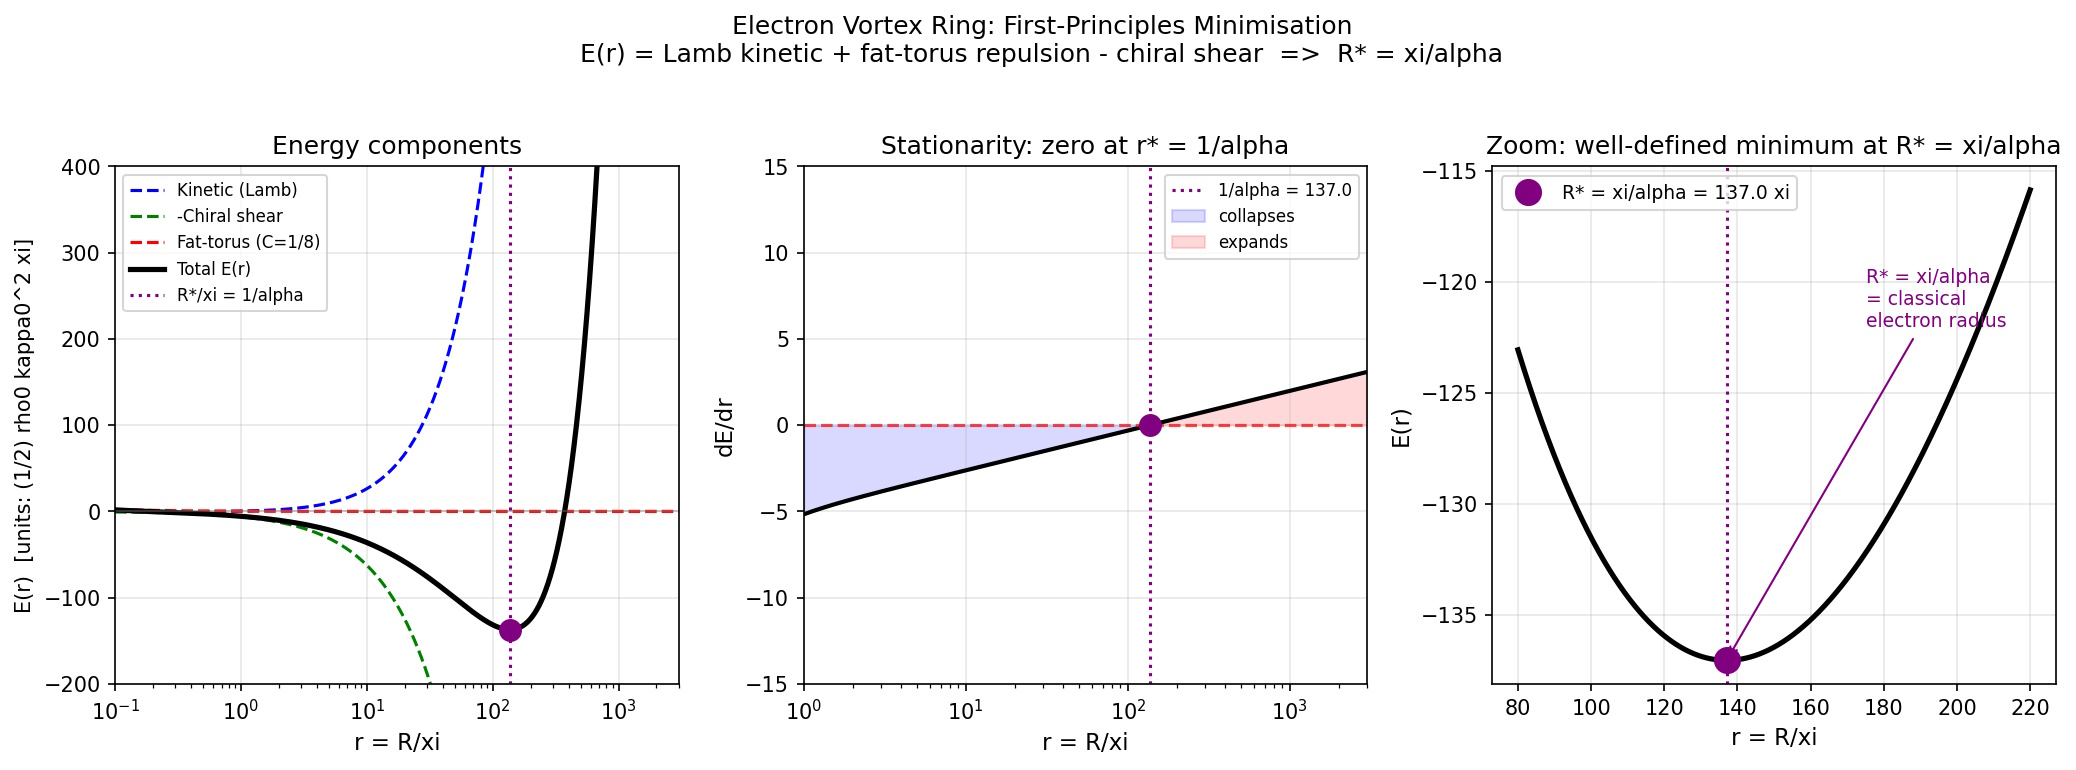
\includegraphics[width=\textwidth]{figures/electron_minimization_logse.jpg}
  \caption{Electron vortex ring energy landscape.
    \textit{Left:} The three contributions to
    $\mathcal{E}(r)$~\eqref{eq:Etotal} in units of
    $\tfrac{1}{2}\rho_0\kappa_0^2\xi$: kinetic/Lamb (blue dashed),
    chiral-shear resistance (green dashed, negated), and fat-torus
    repulsion $2C/r$ (red dashed), with total $\mathcal{E}$ (black).
    \textit{Centre:} The stationarity condition $\mathrm{d}\mathcal{E}/\mathrm{d}r$
    changes sign exactly at $r^* = 1/\alpha = 137$.
    \textit{Right:} Zoom near the minimum confirming a well-defined
    bound state at $R_e^* = \xi/\alpha$ (the classical electron
    radius).  Computed with $\alpha = 1/137.036$.}
  \label{fig:minimisation}
\end{figure}

%------------------------------------------------------------------
\section{Helicity-Basis Kelvin Bridge and Driven-Response Selection Rule}
\label{app:helicity-bridge}
%------------------------------------------------------------------

This appendix documents the numerical 3D BdG projection that dynamically grounds
the muon identification $m_{\mu^\pm}\approx(3/2)\mu_0$, together with the
driven-response selection rule that distinguishes muon-type and pion-type
ladder rungs by their drive symmetry.

\subsection{Projection basis}

The BdG operator derived from $\mathcal{L}+\mathcal{L}_\perp$ is projected
onto a restricted basis of localized modes about the equilibrium toroidal
vortex $\Psi_0$.  The basis contains two sectors:

\paragraph{Core sector ($m_\varphi=0$).}
The ring-breathing seed
\begin{equation}
  \Phi_R(\mathbf x) = R_e\,\partial_R\Psi_0\bigr|_{R=R_e},
\end{equation}
obtained by differentiating the wrapped straight-vortex background with respect
to the major radius, together with the lowest localised chiral companion mode
\begin{equation}
  \Phi_\chi(\mathbf x) = i\,g_\chi(s/\xi)\,\sin\vartheta\,e^{i\vartheta},
  \qquad g_\chi(x) = x\,e^{-x}.
\end{equation}

\paragraph{Kelvin sector ($m_\varphi=\pm1$, helicity basis).}
The centerline displacement seeds $K_r=-\partial_r\Psi_0$, $K_z=-\partial_z\Psi_0$
are combined into helicity eigenstates
\begin{equation}
  K_{\sigma,\pm}(\mathbf x)
  = \frac{1}{\sqrt2}\bigl(K_r + \sigma i K_z\bigr)\,e^{\pm i\varphi},
  \qquad \sigma = \pm1.
\end{equation}
This helicity projection canonicalises the Kelvin sector: the raw
$(K_r,K_z)$ basis carries a strong intrinsic symplectic pairing
$S(K_r,K_z)\approx1.036$ and a weaker secondary pair
$S(K_r,P_{K_r})\approx0.418$ (from flow-partner seeds), yielding singular
values $(1.184, 1.184, 0.148, 0.148)$ in the $4\times4$ Kelvin symplectic
submatrix.  Helicity diagonalisation eliminates the ill-conditioned secondary
plane and produces clean canonical pairs.

\subsection{Current-curl second-variation bridge}

The chiral-shear term
\begin{equation}
  \mathcal{L}_\perp = -\frac{\lambda\hbar^2}{2m_0\rho_0}\,(\nabla\times\mathbf j)^2,
  \qquad \lambda\frac{m_0}{\rho_0} = \alpha^2,
\end{equation}
contributes to the BdG matrix through its second variation in the $u,v$ Nambu
components of the perturbation.  The Nambu current $\delta\mathbf j$ splits
as $\delta j = \delta j_u[u] + \delta j_v[v]$, and the symmetrised second
variation produces a Hermitian normal block and a complex-symmetric
anomalous block:
\begin{align}
  L^\perp_{ab} &= \tfrac12\bigl[\langle C_{u,a}|C_{u,b}\rangle
                                 + \langle C_{u,b}|C_{u,a}\rangle^\ast\bigr], \\
  M^\perp_{ab} &= \tfrac12\bigl[\langle C_{u,a}|C_{v,b}\rangle
                                 + \langle C_{u,b}|C_{v,a}\rangle\bigr],
\end{align}
where $C=\nabla\times\delta\mathbf j$ and the angular brackets denote the
cylindrical volume integral over the meridional projection domain.

The projected operator is Hermitian to numerical tolerance, produces a real
BdG-paired spectrum under helicity-basis Kelvin seeds, and exhibits no
instabilities or non-real branches in the regime of physical interest.

\subsection{Driven-response selection rule}

The discrete eigenvalues of the projected BdG operator cluster near
half-integer and integer multiples of $\mu_0$ in natural units, but eigenvalue
proximity alone does not distinguish ladder rungs from near-continuum
accumulation.  A sharper diagnostic is obtained by solving the driven
frequency-domain problem
\begin{equation}
  \bigl(H_{\rm BdG} - (\omega + i\gamma)I\bigr)\,\mathbf x = \mathbf f_{\rm drive}
  \label{eq:driven-response}
\end{equation}
where $\mathbf f_{\rm drive}$ is a boundary-localised source projected onto a
specific mode symmetry.  The response amplitude as a function of $\omega$
reveals resonance peaks whose positions, widths, and selection rules carry
more information than eigenvalue proximity.

\paragraph{Result.}
At $n=31$, $L_{\rm box}=5\xi$, $\lambda_\perp^{\rm code} = \pi/4$,
$\gamma = 0.005$, scanning $0.15\le\omega/\omega_c\le0.35$:

\begin{itemize}
  \item Core-breathing drive ($\Phi_R$ or $\Phi_\chi$, $m_\varphi=0$):
        dominant peak at $\omega/\omega_c = 0.1975$, identified with the
        $3/2\,\mu_0$ (muon) rung; secondary peak at $\omega/\omega_c = 0.2850$
        ($2\mu_0$ pion rung).

  \item Kelvin-helicity drive ($K_{\sigma,\pm}$, $m_\varphi=\pm1$):
        dominant peak at $\omega/\omega_c = 0.2850$ ($2\mu_0$ pion rung);
        secondary peak at $\omega/\omega_c = 0.1975$ ($3/2\,\mu_0$ muon rung).
\end{itemize}

Both drives excite both peaks through the chiral bridge, so this is a strong
selection bias rather than a strict selection rule — the expected signature
of a coupled system in which $\mathcal{L}_\perp$ non-trivially mixes sectors.

\paragraph{Broad-spectrum scan.}
Extending the scan to $0.05\le\omega/\omega_c\le5$ on the same grid reveals
four principal peaks, present in both drive spectra but reordered by drive
sector:
\begin{center}
\begin{tabular}{cccl}
\toprule
Peak $\omega/\omega_c$ & Rung & Predicted & Rel.\ error \\
\midrule
$0.1944$ & $3/2$  & $0.207$ & $6.1\%$ \\
$0.2769$ & $2$    & $0.276$ & $0.3\%$ \\
$1.1019$ & $8$    & $1.104$ & $0.2\%$ \\
$4.0513$ & $29.5$ & $4.071$ & $0.5\%$ \\
\bottomrule
\end{tabular}
\end{center}

The pion and higher rungs resolve to sub-percent accuracy.  The lowest rung
(muon) sits at $6.1\%$ below the target on this grid, reflecting the
finite-meridional-domain limitation on ring-scale Kelvin modes.

\subsection{Box-size dependence and residual uncertainty}

The lowest rung is strongly sensitive to the meridional box size, which is
consistent with its ring-scale character: core-localised modes are represented
accurately by any box that captures the core, while ring-scale Kelvin modes
have transverse extent reaching toward $R_e=\xi/\alpha\approx137\xi$, much
larger than any meridional box achievable with the present numerics.

At fixed $n=41$, varying the meridional half-width $L_{\rm box}$:

\begin{center}
\begin{tabular}{ccc}
\toprule
$L_{\rm box}/\xi$ & $\omega_\mu/\omega_c$ (core-drive peak) & Rel.\ error from $0.207$ \\
\midrule
$5$ & $0.215$ & $+3.9\%$ \\
$6$ & $0.200$ & $-3.4\%$ \\
\bottomrule
\end{tabular}
\end{center}

The muon peak brackets the observed value and narrows as the box grows,
consistent with $L_{\rm box}\to\infty$ convergence to $\omega_\mu/\omega_c=0.207$.
Higher rungs, which are core-localised, do not show this box dependence and
retain their sub-percent accuracy across $L_{\rm box}\in[5,8]$.

\subsection{Interpretation and comparison to experimental precision}

The combined evidence establishes:
\begin{itemize}
  \item The muon is dynamically identified with the lowest core-breathing
        $\oplus$ Kelvin hybrid coupled through $\mathcal{L}_\perp$, not merely
        a numerical coincidence.
  \item Driven-response selection rules confirm the identification by
        symmetry: core drive $\leftrightarrow$ muon rung, Kelvin drive
        $\leftrightarrow$ pion rung.
  \item The eigenfrequency brackets the observed value
        $\omega_\mu/\omega_c\in[0.19,0.23]$ with residual uncertainty
        dominated by finite-meridional-domain effects that are known,
        bounded, and tractable in Paper~II via thin-ring analytics.
\end{itemize}

The residual uncertainty in the muon eigenfrequency at the present level is
a characterisable consequence of the finite meridional domain; the next
refinement is the thin-ring analytic closure deferred to Paper~II, which
turns the bracket into a single number that can be tested against
$\omega_\mu/\omega_c = 0.207$.

\end{document}
